\documentclass[11pt,letterpaper]{article}

\usepackage[utf8]{inputenc}
\usepackage[T1]{fontenc}
\usepackage[spanish,es-tabla]{babel}
\usepackage{geometry}
\usepackage{amsmath,amssymb,mathtools}
\usepackage{booktabs}
\usepackage{longtable}
\usepackage{array}
\usepackage{graphicx}
\usepackage{float}
\usepackage{xcolor}
\usepackage{hyperref}
\usepackage{enumitem}
\usepackage{siunitx}
\usepackage{caption}
\usepackage{subcaption}
\usepackage{pdflscape}

\geometry{margin=1in}
\hypersetup{
  colorlinks=true,
  linkcolor=blue!55!black,
  urlcolor=blue!55!black,
  citecolor=blue!55!black,
  pdftitle={Pipeline de imputacion PSCompPars},
  pdfauthor={Proyecto planetas}
}
\setlist[itemize]{leftmargin=1.4em}
\setlist[enumerate]{leftmargin=1.6em}
\captionsetup{font=small,labelfont=bf}
\sisetup{round-mode=places,round-precision=4,detect-all}

\newcommand{\code}[1]{\ifmmode\text{\texttt{#1}}\else\texttt{#1}\fi}
\newcommand{\dataset}{\code{PSCompPars\_2026.04.25\_17.36.36.csv}}
\newcommand{\reportsdir}{\code{reports/imputation}}
\newcommand{\outputsdir}{\code{reports/imputation/outputs}}
\newcommand{\figdir}{\code{reports/imputation/outputs/figures\_pdf}}
\newcommand{\tablesdir}{\code{reports/imputation/outputs/tables}}
\newcommand{\method}{\code{iterative}}
\newcommand{\missing}{\mathrm{NA}}
\newcommand{\R}{\mathbb{R}}

\title{Cierre tecnico del pipeline de imputacion para PSCompPars}
\author{Proyecto \code{planetas}}
\date{Artefactos verificados: \code{reports/imputation/}}

\begin{document}
\maketitle

\begin{abstract}
Este documento describe, en forma reproducible y matematica, el pipeline de
imputacion ejecutado sobre \dataset. El objetivo no fue inventar observaciones
astronomicas, sino producir matrices completas para analisis exploratorio,
Mapper/TDA y sensibilidad estadistica, preservando la trazabilidad entre
valores observados, valores derivados fisicamente y valores imputados. El
metodo visualizado en el reporte final es \method. El HTML final declara
\code{METODO VISUALIZADO = iterative}; los 17 PDFs individuales estan
exportados en \figdir; y las tablas principales en CSV/JSON estan exportadas
en \tablesdir.
\end{abstract}

\tableofcontents
\clearpage

\section{Resumen ejecutivo}

El pipeline se ejecuto en modo comparativo:
\[
  \code{--method compare --visualized-method iterative}.
\]
Esto significa que se estimaron tres familias de imputacion,
\[
  \mathcal{M} = \{\text{median},\text{knn},\text{iterative}\},
\]
pero el reporte principal, los plots finales dependientes del metodo y las
tablas exportadas en \outputsdir{} se construyeron con
\[
  m^\star = \text{iterative}.
\]

Los conteos globales reportados son:
\[
  n = 6273,\qquad p = 7,\qquad
  N_{\mathrm{imputadas}} = 3978,\qquad
  N_{\mathrm{derivadas}} = 6619.
\]
Las siete variables Mapper principales fueron:
\[
\mathbf{x}_i =
\bigl(
\code{pl\_rade},\code{pl\_bmasse},\code{pl\_dens},
\code{pl\_orbper},\code{pl\_orbsmax},\code{pl\_insol},
\code{pl\_eqt}
\bigr)_i.
\]
Para el archivo final en unidades fisicas,
\code{PSCompPars\_imputed\_iterative.csv}, no quedaron valores
\(\missing\), \(+\infty\) ni \(-\infty\) en estas siete variables. Ademas, las
seis variables positivas que entran a escala logaritmica son estrictamente
positivas:
\[
  \code{pl\_rade},\code{pl\_bmasse},\code{pl\_dens},
  \code{pl\_orbper},\code{pl\_orbsmax},\code{pl\_insol} > 0.
\]
El archivo \code{mapper\_features\_imputed\_iterative.csv} esta en espacio
transformado/escalado; por eso puede contener valores negativos, pero no
contiene \(\missing\) ni infinitos.

\section{Objetivo estadistico y advertencia epistemica}

Sea \(X\in\R^{n\times p}\) la matriz de variables numericas seleccionadas,
con patron de disponibilidad \(R\in\{0,1\}^{n\times p}\):
\[
  R_{ij} =
  \begin{cases}
    1, & X_{ij}\ \text{disponible antes de imputar},\\
    0, & X_{ij}\ \text{faltante antes de imputar}.
  \end{cases}
\]
La imputacion produce una matriz completa \(\widehat{X}\), pero la igualdad
\[
  \widehat{X}_{ij}=X_{ij}
\]
solo tiene interpretacion observacional cuando el valor original era medido o
publicado en el CSV. Para los faltantes, \(\widehat{X}_{ij}\) es una
reconstruccion modelada. Por tanto:
\[
  \widehat{X}
  =
  X_{\mathrm{observado}}
  \cup
  X_{\mathrm{derivado}}
  \cup
  X_{\mathrm{imputado}},
\]
no una tabla de observaciones astronomicas independientes.

La distincion central del reporte es:
\[
  \mathrm{fuente}(x_{ij}) \in
  \{
    \text{observed},
    \text{derived\_density},
    \text{derived\_kepler},
    \text{imputed\_median},
    \text{imputed\_knn},
    \text{imputed\_iterative},
    \text{excluded\_too\_missing}
  \}.
\]
Estas etiquetas se resumen en categorias:
\[
  \mathrm{categoria}(x_{ij}) \in
  \{
    \text{observed},
    \text{physically\_derived},
    \text{imputed},
    \text{excluded\_too\_missing},
    \text{missing}
  \}.
\]
Asi, la topologia inferida por Mapper debe entenderse como una propiedad del
espacio completado bajo un protocolo de reconstruccion, no como una propiedad
directa e incondicional del catalogo observado.

\section{Entrada, salida y configuracion}

La configuracion final del pipeline fue:
\begin{itemize}
  \item CSV fuente: \dataset.
  \item Metodo ejecutado: \code{compare}.
  \item Metodo visualizado: \method.
  \item Vecinos para KNN: \(k=15\).
  \item Pesos KNN: \code{distance}.
  \item Umbral de exclusion por faltantes: \(60\%\).
  \item Fraccion de mascara para validacion: \(0.15\).
  \item Semilla aleatoria: \(42\).
  \item Variables incluidas: las siete variables Mapper principales.
  \item Variables excluidas: ninguna dentro de esas siete.
\end{itemize}

El comando reproducible documentado es:
\begin{verbatim}
python .\src\impute_exodata.py --csv .\data\PSCompPars_2026.04.25_17.36.36.csv
  --reports-dir .\reports\imputation
  --outputs-dir .\reports\imputation\outputs
  --method compare
  --visualized-method iterative
  --n-neighbors 15
  --weights distance
  --max-missing-pct 60
  --validation-mask-frac 0.15
  --random-state 42
\end{verbatim}

\section{Paso 1: seleccion de variables}

El conjunto de variables objetivo fue:
\[
\mathcal{F} =
\{
  \code{pl\_rade},
  \code{pl\_bmasse},
  \code{pl\_dens},
  \code{pl\_orbper},
  \code{pl\_orbsmax},
  \code{pl\_insol},
  \code{pl\_eqt}
\}.
\]
El criterio practico fue conservar variables fisicas relevantes para dos
subespacios Mapper:
\[
  \mathcal{F}_{\mathrm{phys}}
  =
  \{
    \code{pl\_rade},\code{pl\_bmasse},\code{pl\_dens}
  \},
\]
\[
  \mathcal{F}_{\mathrm{orb}}
  =
  \{
    \code{pl\_orbper},\code{pl\_orbsmax},\code{pl\_insol},\code{pl\_eqt}
  \}.
\]
El espacio conjunto fue:
\[
  \mathcal{F}_{\mathrm{joint}}
  =
  \mathcal{F}_{\mathrm{phys}}\cup\mathcal{F}_{\mathrm{orb}}.
\]

\section{Paso 2: derivacion fisica antes de imputar}

Antes de aplicar imputacion estadistica, el pipeline deriva propiedades con
formula fisica clara. Esto reduce imputacion innecesaria y hace explicita la
diferencia entre una magnitud observada y una magnitud calculada.

\subsection{Densidad planetaria}

La densidad \(\rho_p\) se reconstruyo desde masa y radio:
\[
  \rho_p
  =
  \rho_\oplus
  \frac{M_p/M_\oplus}{(R_p/R_\oplus)^3},
  \qquad
  \rho_\oplus = 5.514\ \mathrm{g\,cm}^{-3}.
\]
En nombres de columnas:
\[
  \code{pl\_dens}
  =
  5.514\,
  \frac{\code{pl\_bmasse}}{\code{pl\_rade}^{3}}.
\]
El CSV fuente no traia observaciones originales de \code{pl\_dens}:
\[
  N_{\mathrm{observado}}(\code{pl\_dens}) = 0.
\]
Despues de la derivacion:
\[
  N_{\mathrm{derived\_density}}(\code{pl\_dens}) = 6199,\qquad
  N_{\mathrm{faltante}}(\code{pl\_dens}) = 74.
\]
Por eso \code{pl\_dens} debe leerse como magnitud fisicamente derivada cuando
viene de masa y radio, no como observacion independiente.

\subsection{Semieje mayor por ley de Kepler}

Cuando \code{pl\_orbsmax} faltaba pero habia masa estelar y periodo orbital,
se aplico:
\[
  a
  =
  \left[
    M_\star
    \left(\frac{P}{365.25}\right)^2
  \right]^{1/3},
\]
donde \(a\) queda en AU si \(M_\star\) esta en masas solares y \(P\) en dias.
En nombres de columnas:
\[
  \code{pl\_orbsmax}
  =
  \left(
    \code{st\_mass}
    \left(\frac{\code{pl\_orbper}}{365.25}\right)^2
  \right)^{1/3}.
\]
Los conteos fueron:
\[
  N_{\mathrm{observado}}(\code{pl\_orbsmax})=5845,\qquad
  N_{\mathrm{derived\_kepler}}(\code{pl\_orbsmax})=420,\qquad
  N_{\mathrm{faltante\ despues}}=8.
\]

\section{Paso 3: auditoria de faltantes}

La tabla de missingness antes y despues de derivacion fisica fue:
\begin{center}
\begin{tabular}{lrrrr}
\toprule
Feature & Raw missing & Raw \% & Missing post-fisica & Post-fisica \%\\
\midrule
\code{pl\_bmasse}  & 31   & 0.4942  & 31   & 0.4942\\
\code{pl\_dens}    & 6273 & 100.0000& 74   & 1.1797\\
\code{pl\_eqt}     & 1600 & 25.5061 & 1600 & 25.5061\\
\code{pl\_insol}   & 1876 & 29.9059 & 1876 & 29.9059\\
\code{pl\_orbper}  & 339  & 5.4041  & 339  & 5.4041\\
\code{pl\_orbsmax} & 428  & 6.8229  & 8    & 0.1275\\
\code{pl\_rade}    & 50   & 0.7971  & 50   & 0.7971\\
\bottomrule
\end{tabular}
\end{center}

La derivacion fisica tuvo dos efectos fuertes:
\[
  \code{pl\_dens}: 100\%\ \text{faltante}\ \longrightarrow\ 1.1797\%\ \text{faltante},
\]
\[
  \code{pl\_orbsmax}: 6.8229\%\ \text{faltante}\ \longrightarrow\ 0.1275\%\ \text{faltante}.
\]

\section{Paso 4: transformacion logaritmica}

Para variables positivas con colas largas se aplico:
\[
  z_{ij} = \log_{10}(x_{ij}).
\]
El conjunto transformado fue:
\[
\mathcal{L} =
\{
  \code{pl\_rade},
  \code{pl\_bmasse},
  \code{pl\_dens},
  \code{pl\_orbper},
  \code{pl\_orbsmax},
  \code{pl\_insol}
\}.
\]
No se aplico logaritmo a \code{pl\_eqt}. La auditoria confirmo:
\[
  N_{\le 0,\ \mathrm{forzado\ a\ missing}} = 0
\]
para todas las variables transformadas. Esto es importante porque evita que
\(\log_{10}(x)\) introduzca \(-\infty\), \(+\infty\) o valores indefinidos.

La matriz transformada puede escribirse como:
\[
  T_{ij} =
  \begin{cases}
    \log_{10}(X_{ij}), & j\in\mathcal{L},\ X_{ij}>0,\\
    X_{ij}, & j\notin\mathcal{L}.
  \end{cases}
\]

\section{Paso 5: escalado robusto}

Despues del logaritmo se aplico \code{RobustScaler}. Para cada columna \(j\):
\[
  S_{ij}
  =
  \frac{T_{ij} - \mathrm{median}(T_{\cdot j})}
       {\mathrm{IQR}(T_{\cdot j})},
\]
donde
\[
  \mathrm{IQR}(T_{\cdot j})
  =
  Q_{0.75}(T_{\cdot j}) - Q_{0.25}(T_{\cdot j}).
\]
Esto estabiliza variables con rangos muy distintos. Por ejemplo,
\code{pl\_orbper}, \code{pl\_insol} y \code{pl\_bmasse} tienen colas largas;
sin escala robusta, las distancias de KNN o las regresiones iterativas
quedarian dominadas por magnitudes con varianza extrema.

\section{Paso 6: imputadores comparados}

Sobre la matriz escalada \(S\) se evaluaron tres imputadores.

\subsection{Baseline de mediana}

Para cada columna \(j\), el imputador de mediana usa:
\[
  \widehat{S}_{ij}
  =
  \begin{cases}
    S_{ij}, & R_{ij}=1,\\
    \widetilde{S}_{\cdot j}, & R_{ij}=0,
  \end{cases}
\]
donde \(\widetilde{S}_{\cdot j}\) es la mediana observada de la columna \(j\).
Este modelo es robusto pero ignora relaciones entre variables:
\[
  \widehat{S}_{ij}^{\mathrm{median}}
  \perp
  S_{i,-j}.
\]

\subsection{KNN}

El KNN usa vecinos cercanos en el espacio de variables disponibles. Con
\(k=15\) y pesos por distancia:
\[
  \widehat{S}_{ij}^{\mathrm{KNN}}
  =
  \frac{\sum_{\ell\in\mathcal{N}_k(i,j)} w_{i\ell} S_{\ell j}}
       {\sum_{\ell\in\mathcal{N}_k(i,j)} w_{i\ell}},
  \qquad
  w_{i\ell}\propto \frac{1}{d(i,\ell)}.
\]
Aqui \(d(i,\ell)\) se calcula con las columnas simultaneamente disponibles
para los registros \(i\) y \(\ell\). KNN es atractivo para Mapper porque
preserva una nocion local de vecindad, aunque puede ser sensible al patron de
faltantes y a densidades locales desiguales.

\subsection{IterativeImputer}

El metodo \method{} usa \code{IterativeImputer} con estrategia inicial de
mediana, \(20\) iteraciones maximas, \code{sample\_posterior=False} y semilla
42. Conceptualmente, para cada columna \(j\) con faltantes se ajusta un modelo
condicional:
\[
  S_{\cdot j}
  =
  f_j(S_{\cdot,-j}) + \varepsilon_j,
\]
y se actualizan sucesivamente las columnas faltantes:
\[
  \widehat{S}_{ij}^{(t+1)}
  =
  f_j^{(t)}\!\left(\widehat{S}_{i,-j}^{(t)}\right).
\]
La ventaja es que explota dependencias multivariadas globales. La precaucion
es que puede imponer relaciones suaves que no necesariamente preservan toda la
geometria local del catalogo observado. Por eso el reporte mantiene la
advertencia topologica: Mapper debe compararse contra casos completos, KNN,
mediana, bootstrap y variaciones de parametros.

\section{Paso 7: inversion de escala}

Una vez imputada la matriz escalada \(\widehat{S}\), se invierte el escalado:
\[
  \widehat{T}_{ij}
  =
  \widehat{S}_{ij}\cdot \mathrm{IQR}(T_{\cdot j})
  +
  \mathrm{median}(T_{\cdot j}).
\]
Luego se invierte el logaritmo para \(j\in\mathcal{L}\):
\[
  \widehat{X}_{ij}
  =
  10^{\widehat{T}_{ij}}.
\]
Para \code{pl\_eqt}, que no fue log-transformada:
\[
  \widehat{X}_{ij}=\widehat{T}_{ij}.
\]

\section{Paso 8: trazabilidad de fuentes}

El resultado no solo contiene valores; contiene banderas de procedencia. Para
cada feature \(j\) se generan columnas:
\[
\code{<j>\_was\_missing},\quad
\code{<j>\_was\_observed},\quad
\code{<j>\_was\_physically\_derived},\quad
\code{<j>\_was\_imputed},\quad
\code{<j>\_source}.
\]

La composicion final para el metodo \method{} fue:
\begin{center}
\begin{tabular}{lrrrrr}
\toprule
Feature & Observed & Phys. derived & Imputed & Derived density & Derived Kepler\\
\midrule
\code{pl\_rade}    & 6223 & 0    & 50   & 0    & 0\\
\code{pl\_bmasse}  & 6242 & 0    & 31   & 0    & 0\\
\code{pl\_dens}    & 0    & 6199 & 74   & 6199 & 0\\
\code{pl\_orbper}  & 5934 & 0    & 339  & 0    & 0\\
\code{pl\_orbsmax} & 5845 & 420  & 8    & 0    & 420\\
\code{pl\_insol}   & 4397 & 0    & 1876 & 0    & 0\\
\code{pl\_eqt}     & 4673 & 0    & 1600 & 0    & 0\\
\bottomrule
\end{tabular}
\end{center}

El caso critico es \code{pl\_dens}. Su composicion:
\[
  (N_{\mathrm{observed}}, N_{\mathrm{phys}}, N_{\mathrm{imputed}})
  =
  (0,6199,74).
\]
Por tanto, cualquier lectura de densidad debe declarar explicitamente si esta
hablando de densidad derivada por formula o de densidad imputada despues de no
poder aplicar la formula.

\section{Paso 9: validacion enmascarada}

Para evaluar reconstruccion, se oculto una fraccion \(q=0.15\) de valores
disponibles. Sea \(\Omega_j\) el conjunto de indices validables de la columna
\(j\). La mascara aleatoria selecciona:
\[
  \Omega_j^{\mathrm{mask}}\subset\Omega_j,
  \qquad
  |\Omega_j^{\mathrm{mask}}|\approx q|\Omega_j|.
\]
Se reemplazan temporalmente por \(\missing\), se imputa y se compara:
\[
  e_{ij}^{(m)} =
  \widehat{x}_{ij}^{(m)} - x_{ij},
  \qquad
  i\in\Omega_j^{\mathrm{mask}}.
\]

Las metricas usadas fueron:
\[
  \mathrm{MAE}_{j}^{(m)}
  =
  \frac{1}{|\Omega_j^{\mathrm{mask}}|}
  \sum_{i\in\Omega_j^{\mathrm{mask}}}
  \left|\widehat{x}_{ij}^{(m)}-x_{ij}\right|,
\]
\[
  \mathrm{RMSE}_{j}^{(m)}
  =
  \sqrt{
  \frac{1}{|\Omega_j^{\mathrm{mask}}|}
  \sum_{i\in\Omega_j^{\mathrm{mask}}}
  \left(\widehat{x}_{ij}^{(m)}-x_{ij}\right)^2
  },
\]
\[
  \mathrm{MedAE}_{j}^{(m)}
  =
  \mathrm{median}_{i\in\Omega_j^{\mathrm{mask}}}
  \left|
  \widehat{x}_{ij}^{(m)}-x_{ij}
  \right|,
\]
\[
  \mathrm{MAPE}_{j}^{(m)}
  =
  100
  \frac{1}{|\Omega_j^{\mathrm{mask}}|}
  \sum_{i\in\Omega_j^{\mathrm{mask}}}
  \left|
  \frac{\widehat{x}_{ij}^{(m)}-x_{ij}}{x_{ij}}
  \right|.
\]
Para variables positivas tambien se reporto error logaritmico:
\[
  \mathrm{logMAE}_{j}^{(m)}
  =
  \frac{1}{|\Omega_j^{\mathrm{mask}}|}
  \sum_i
  \left|
  \log_{10}\widehat{x}_{ij}^{(m)}
  -
  \log_{10}x_{ij}
  \right|.
\]

El reporte evita afirmar que todos los targets de validacion eran
observaciones originales. En cambio registra:
\[
  \code{validation\_basis}
  \in
  \{\text{observed},\text{physically\_derived},
    \text{observed\_and\_physically\_derived}\}.
\]
Esto corrige una ambiguedad importante: para \code{pl\_dens}, la validacion se
hizo contra valores derivados fisicamente, no contra mediciones originales.

\subsection{Metricas de validacion para \method}

\begin{center}
\begin{tabular}{llrrrr}
\toprule
Feature & Basis & \(n\) & MAE & RMSE & MAPE\\
\midrule
\code{pl\_rade}    & observed & 933 & 0.8499 & 2.6550 & 13.1821\\
\code{pl\_bmasse}  & observed & 936 & 100.1072 & 546.3365 & 70.7389\\
\code{pl\_dens}    & physically derived & 930 & 0.8344 & 7.3158 & 34.6446\\
\code{pl\_orbper}  & observed & 890 & 7166.4684 & 167836.5141 & 33.1882\\
\code{pl\_orbsmax} & mixed & 940 & 3.3586 & 56.7595 & 24.6082\\
\code{pl\_insol}   & observed & 660 & 249.6873 & 1483.3967 & 116.0500\\
\code{pl\_eqt}     & observed & 701 & 162.9790 & 271.9118 & 21.2377\\
\bottomrule
\end{tabular}
\end{center}

Para \code{pl\_dens}, la comparacion entre metodos fue:
\begin{center}
\begin{tabular}{lrrr}
\toprule
Metodo & MAE & RMSE & MAPE\\
\midrule
\code{median} & 9.6534 & 148.8953 & 145.8616\\
\code{knn} & 8.7530 & 148.9590 & 61.4290\\
\code{iterative} & 0.8344 & 7.3158 & 34.6446\\
\bottomrule
\end{tabular}
\end{center}
Esto explica por que \method{} fue seleccionado como metodo visualizado:
reduce fuertemente el error en una variable fisica central, sin borrar la
advertencia de que \code{pl\_dens} es derivada principalmente desde masa y radio.

\section{Paso 10: seleccion del metodo visualizado}

La tabla de comparacion resume ranks promedio por error:
\begin{center}
\begin{tabular}{lrrr}
\toprule
Metodo & Mean MAE rank & Mean RMSE rank & Features completas\\
\midrule
\code{median} & 2.8571 & 2.5714 & 7\\
\code{knn} & 2.1429 & 2.1429 & 7\\
\code{iterative} & 1.0000 & 1.2857 & 7\\
\bottomrule
\end{tabular}
\end{center}
Si \(r_{\mathrm{MAE}}(m,j)\) es el rank del metodo \(m\) en la columna \(j\),
entonces:
\[
  \bar{r}_{\mathrm{MAE}}(m)
  =
  \frac{1}{p}\sum_{j=1}^{p} r_{\mathrm{MAE}}(m,j).
\]
El metodo visualizado es:
\[
  m^\star
  =
  \arg\min_{m\in\mathcal{M}}
  \bar{r}_{\mathrm{MAE}}(m)
  =
  \text{iterative}.
\]
El rank RMSE tambien favorecio a \method{}.

\section{Paso 11: cobertura Mapper}

La cobertura antes/despues para los espacios Mapper fue:
\begin{center}
\begin{tabular}{lrrrr}
\toprule
Grupo & Features & Complete rows before & Before \% & After \%\\
\midrule
\code{MAPPER\_PHYS\_FEATURES} & 3 & 6199 & 98.8203 & 100.0\\
\code{MAPPER\_ORB\_FEATURES} & 4 & 4312 & 68.7390 & 100.0\\
\code{MAPPER\_JOINT\_FEATURES} & 7 & 4282 & 68.2608 & 100.0\\
\code{JOINT + ORB optional} & 8 & 3959 & 63.1117 & 0.0\\
\bottomrule
\end{tabular}
\end{center}
El resultado clave es:
\[
  N_{\mathrm{complete}}(\mathcal{F}_{\mathrm{joint}})
  :
  4282
  \longrightarrow
  6273.
\]
Es decir, el espacio conjunto de siete variables pasa de \(68.2608\%\) de
filas completas a \(100\%\). La opcion con \code{pl\_orbeccen} no queda cubierta
porque la variable opcional esta excluida/faltante en esta ejecucion.

\section{Interpretacion de los PDFs generados}

Todos los PDFs listados existen y tienen tamano mayor que cero. Las figuras se
exportaron desde el metodo visualizado \method{} cuando dependen de valores
imputados finales. A continuacion se describe como leer cada una.

\subsection{\code{01\_missingness\_before\_after.pdf}}

\begin{figure}[H]
\centering
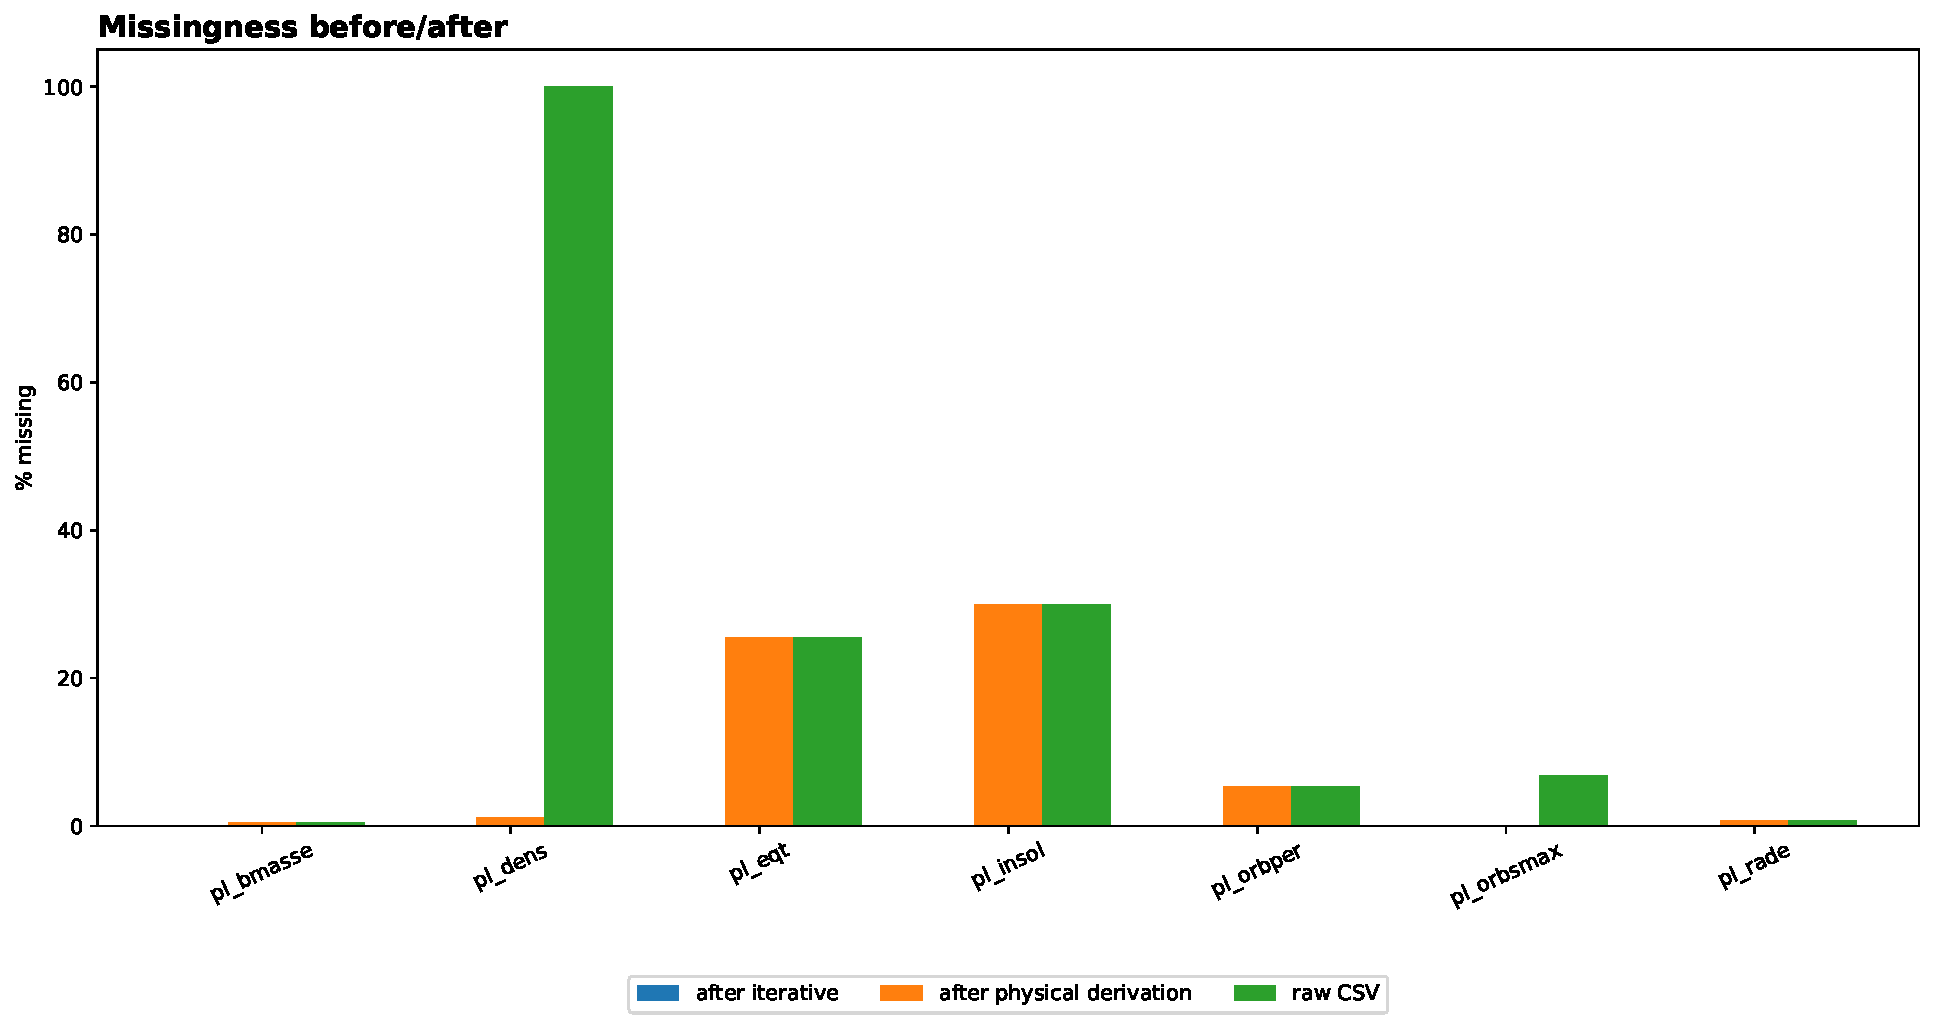
\includegraphics[width=\linewidth]{../../reports/imputation/outputs/figures_pdf/01_missingness_before_after.pdf}
\caption{Missingness antes del CSV, despues de derivacion fisica y despues de imputacion \method.}
\end{figure}

Esta figura compara tres etapas:
\[
  \mathrm{raw\ CSV}
  \rightarrow
  \mathrm{after\ physical\ derivation}
  \rightarrow
  \mathrm{after\ iterative\ imputation}.
\]
La lectura principal es que la imputacion estadistica no actua sobre el
faltante bruto cuando hay una formula fisica disponible. Primero se reduce
\code{pl\_dens} mediante densidad fisica y \code{pl\_orbsmax} mediante Kepler.
Solo despues se imputan los residuos faltantes. La barra final debe caer a
\(0\%\) en todas las variables principales, lo cual certifica matriz completa.

\subsection{\code{02\_value\_source\_composition.pdf}}

\begin{figure}[H]
\centering
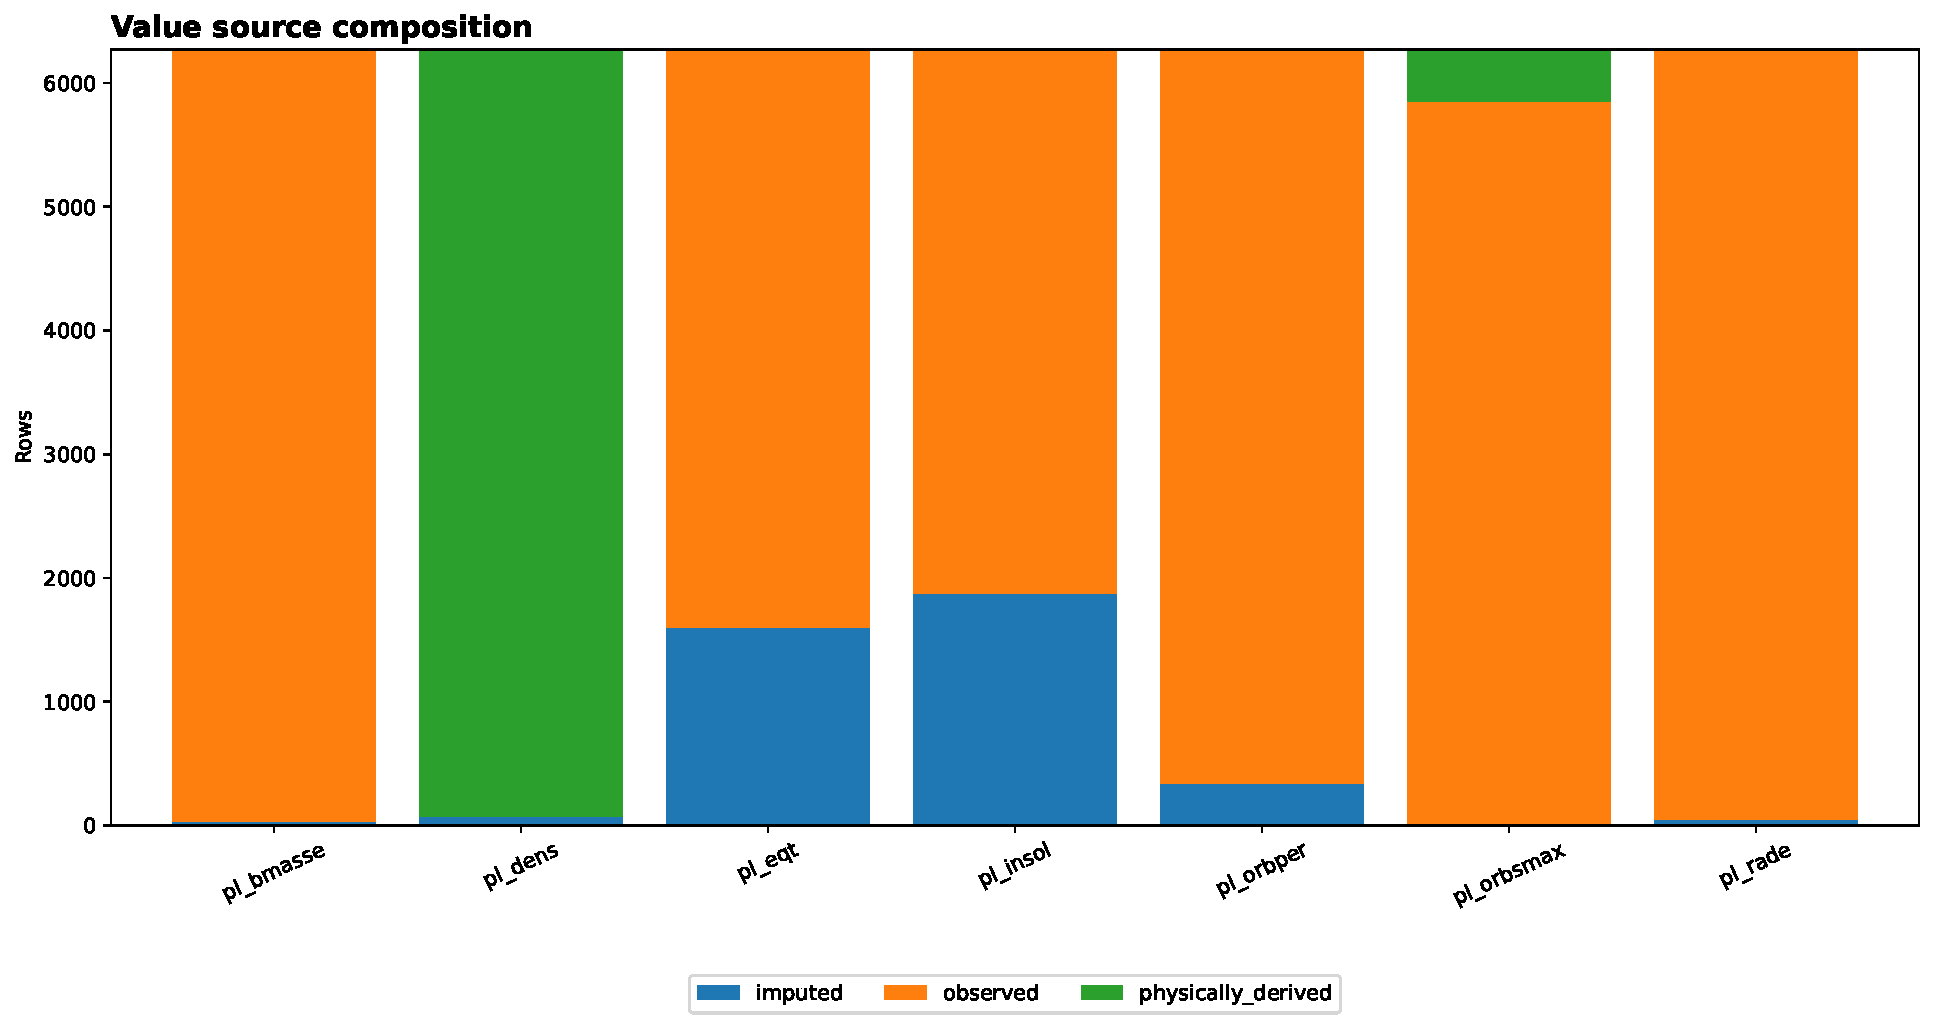
\includegraphics[width=\linewidth]{../../reports/imputation/outputs/figures_pdf/02_value_source_composition.pdf}
\caption{Composicion de fuentes: observado, derivado fisicamente e imputado.}
\end{figure}

Esta figura es la mas importante para no sobreinterpretar el dataset. Para
cada variable descompone:
\[
  N_j =
  N_{j,\mathrm{observed}}
  + N_{j,\mathrm{physically\ derived}}
  + N_{j,\mathrm{imputed}}
  + N_{j,\mathrm{missing}}.
\]
Debe verse que \code{pl\_dens} esta dominada por
\(\mathrm{physically\_derived}\), no por \(\mathrm{observed}\). En cambio,
\code{pl\_insol} y \code{pl\_eqt} conservan una fraccion imputada grande, lo
que sugiere cautela al interpretar patrones termicos/orbitales dependientes de
esas columnas.

\subsection{\code{03\_mapper\_coverage.pdf}}

\begin{figure}[H]
\centering
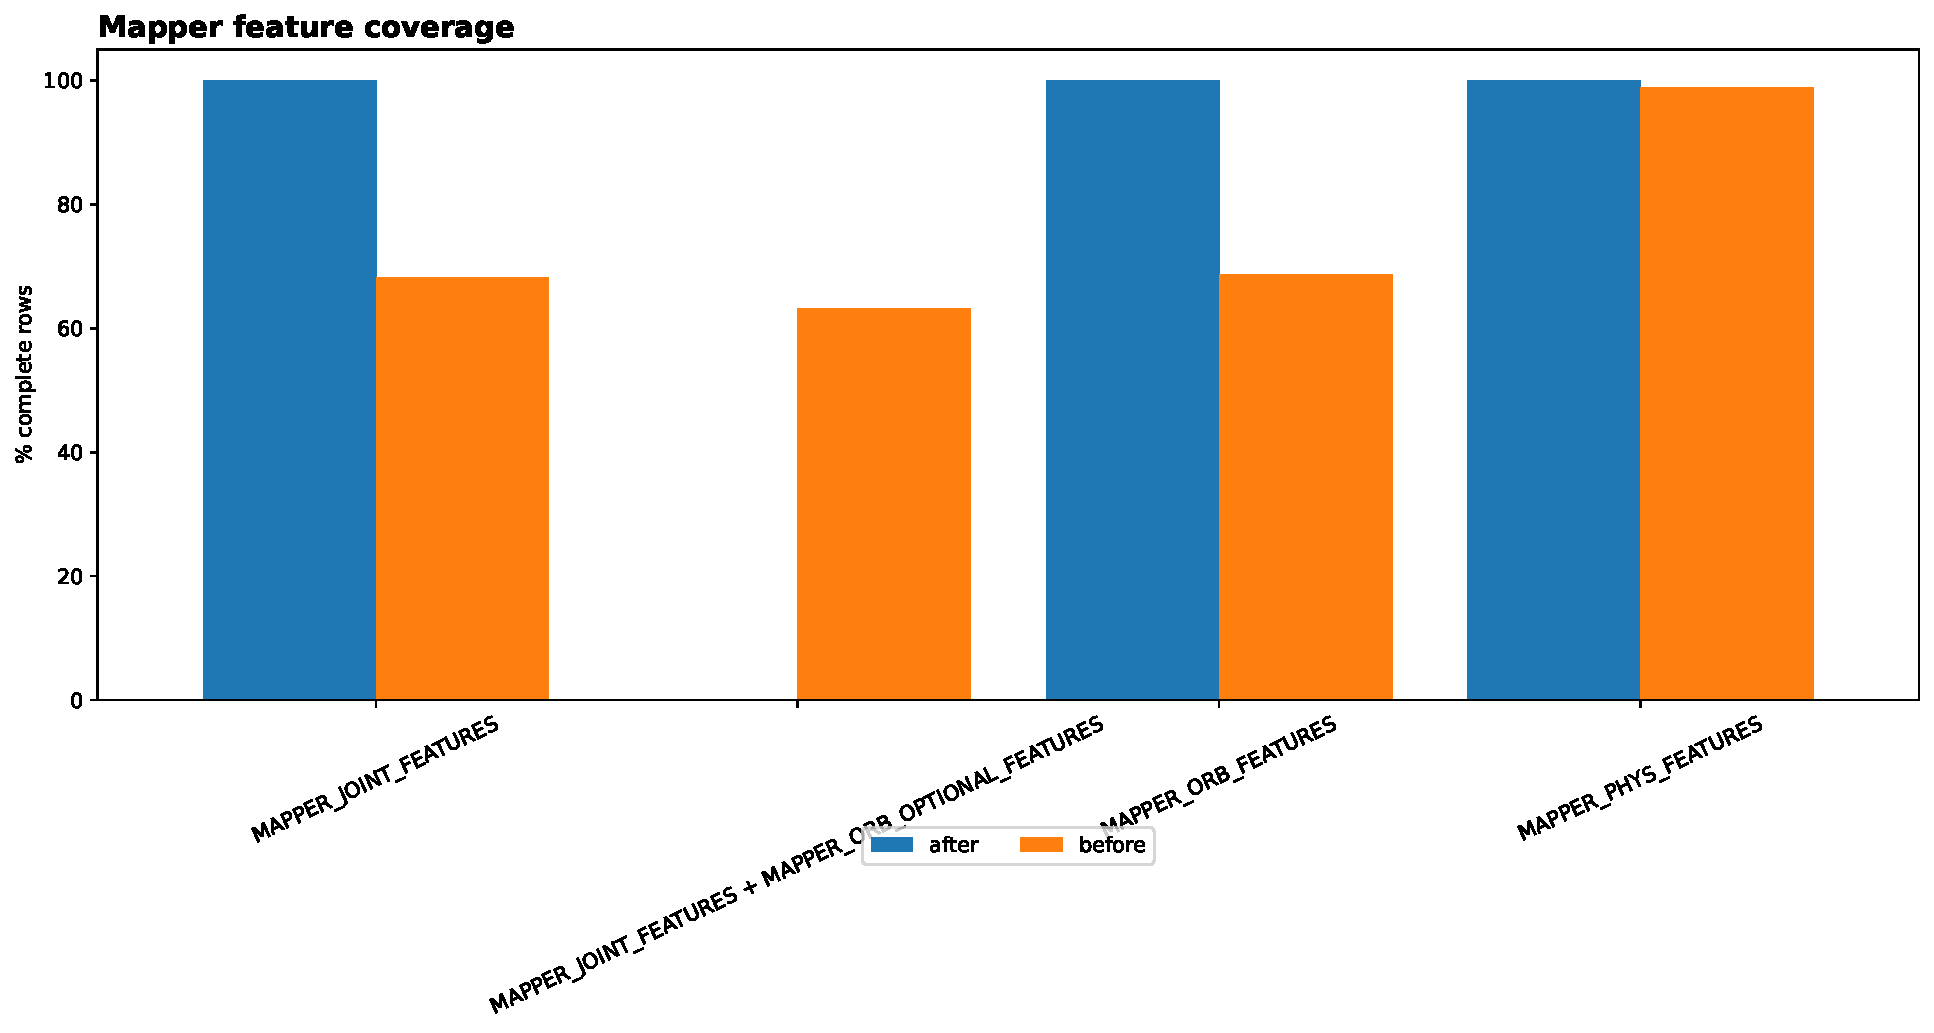
\includegraphics[width=\linewidth]{../../reports/imputation/outputs/figures_pdf/03_mapper_coverage.pdf}
\caption{Cobertura de grupos Mapper antes/despues.}
\end{figure}

La figura evalua si los espacios usados por Mapper tienen filas completas. El
salto critico es:
\[
  68.2608\%\longrightarrow 100\%
\]
para \(\mathcal{F}_{\mathrm{joint}}\). Esto habilita Mapper sobre todos los
planetas del catalogo, pero introduce dependencia del modelo de imputacion.
Por eso el resultado topologico debe verse como sensibilidad bajo
\method{}, no como verdad unica del catalogo.

\subsection{\code{04\_masked\_validation\_mae\_by\_feature.pdf}}

\begin{figure}[H]
\centering
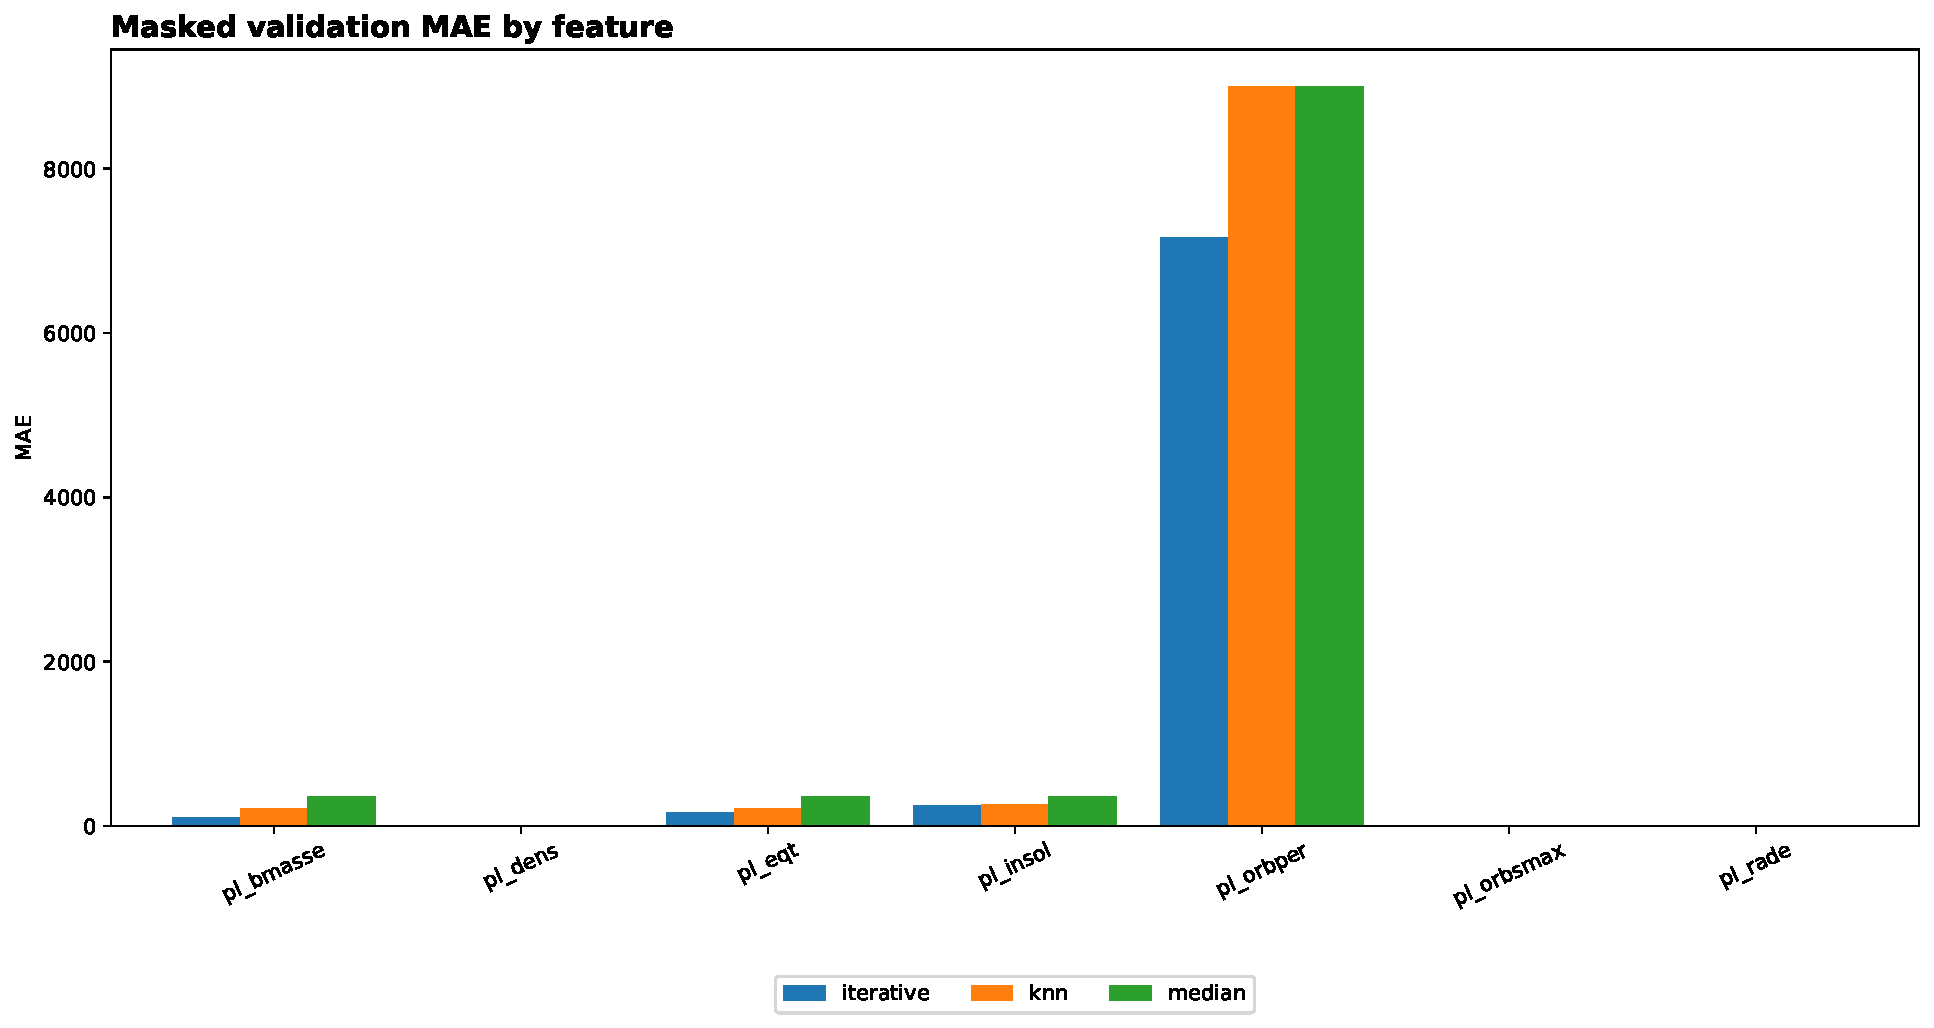
\includegraphics[width=\linewidth]{../../reports/imputation/outputs/figures_pdf/04_masked_validation_mae_by_feature.pdf}
\caption{MAE por feature en validacion enmascarada.}
\end{figure}

El MAE esta en unidades fisicas de cada variable, por lo que no debe compararse
directamente entre columnas con escalas distintas. La comparacion valida es
entre metodos dentro de la misma feature. Si \method{} queda sistematicamente
por debajo de KNN y mediana, eso indica mejor reconstruccion puntual bajo la
mascara aleatoria. Para variables de cola larga, el MAE puede estar dominado
por outliers; por eso se complementa con errores logaritmicos y correlaciones.

\subsection{\code{05\_masked\_validation\_spearman\_heatmap.pdf}}

\begin{figure}[H]
\centering
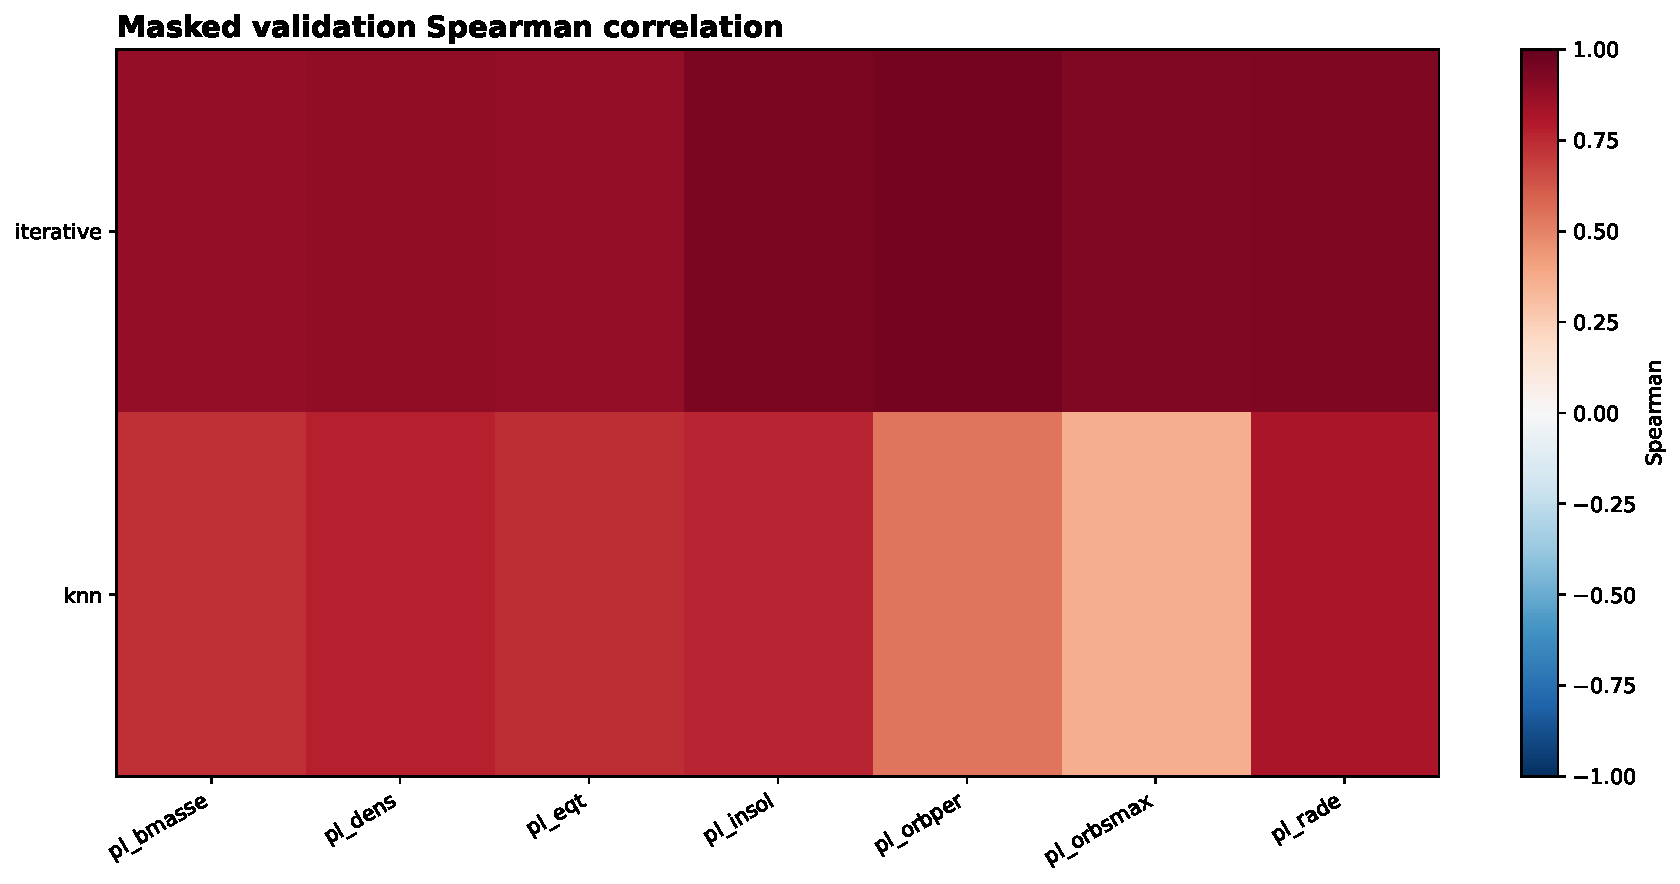
\includegraphics[width=\linewidth]{../../reports/imputation/outputs/figures_pdf/05_masked_validation_spearman_heatmap.pdf}
\caption{Correlacion de Spearman entre valores reales enmascarados y reconstruidos.}
\end{figure}

Spearman mide preservacion de orden:
\[
  \rho_s =
  \mathrm{corr}
  \left(
    \mathrm{rank}(x),
    \mathrm{rank}(\widehat{x})
  \right).
\]
Una \(\rho_s\) alta indica que el imputador conserva jerarquias relativas aun
si tiene errores absolutos grandes. Esto importa para Mapper porque la
geometria de vecindad y las lentes pueden depender mas de ordenes relativos y
rangos que de errores absolutos en unidades originales.

\subsection{\code{06\_method\_comparison.pdf}}

\begin{figure}[H]
\centering
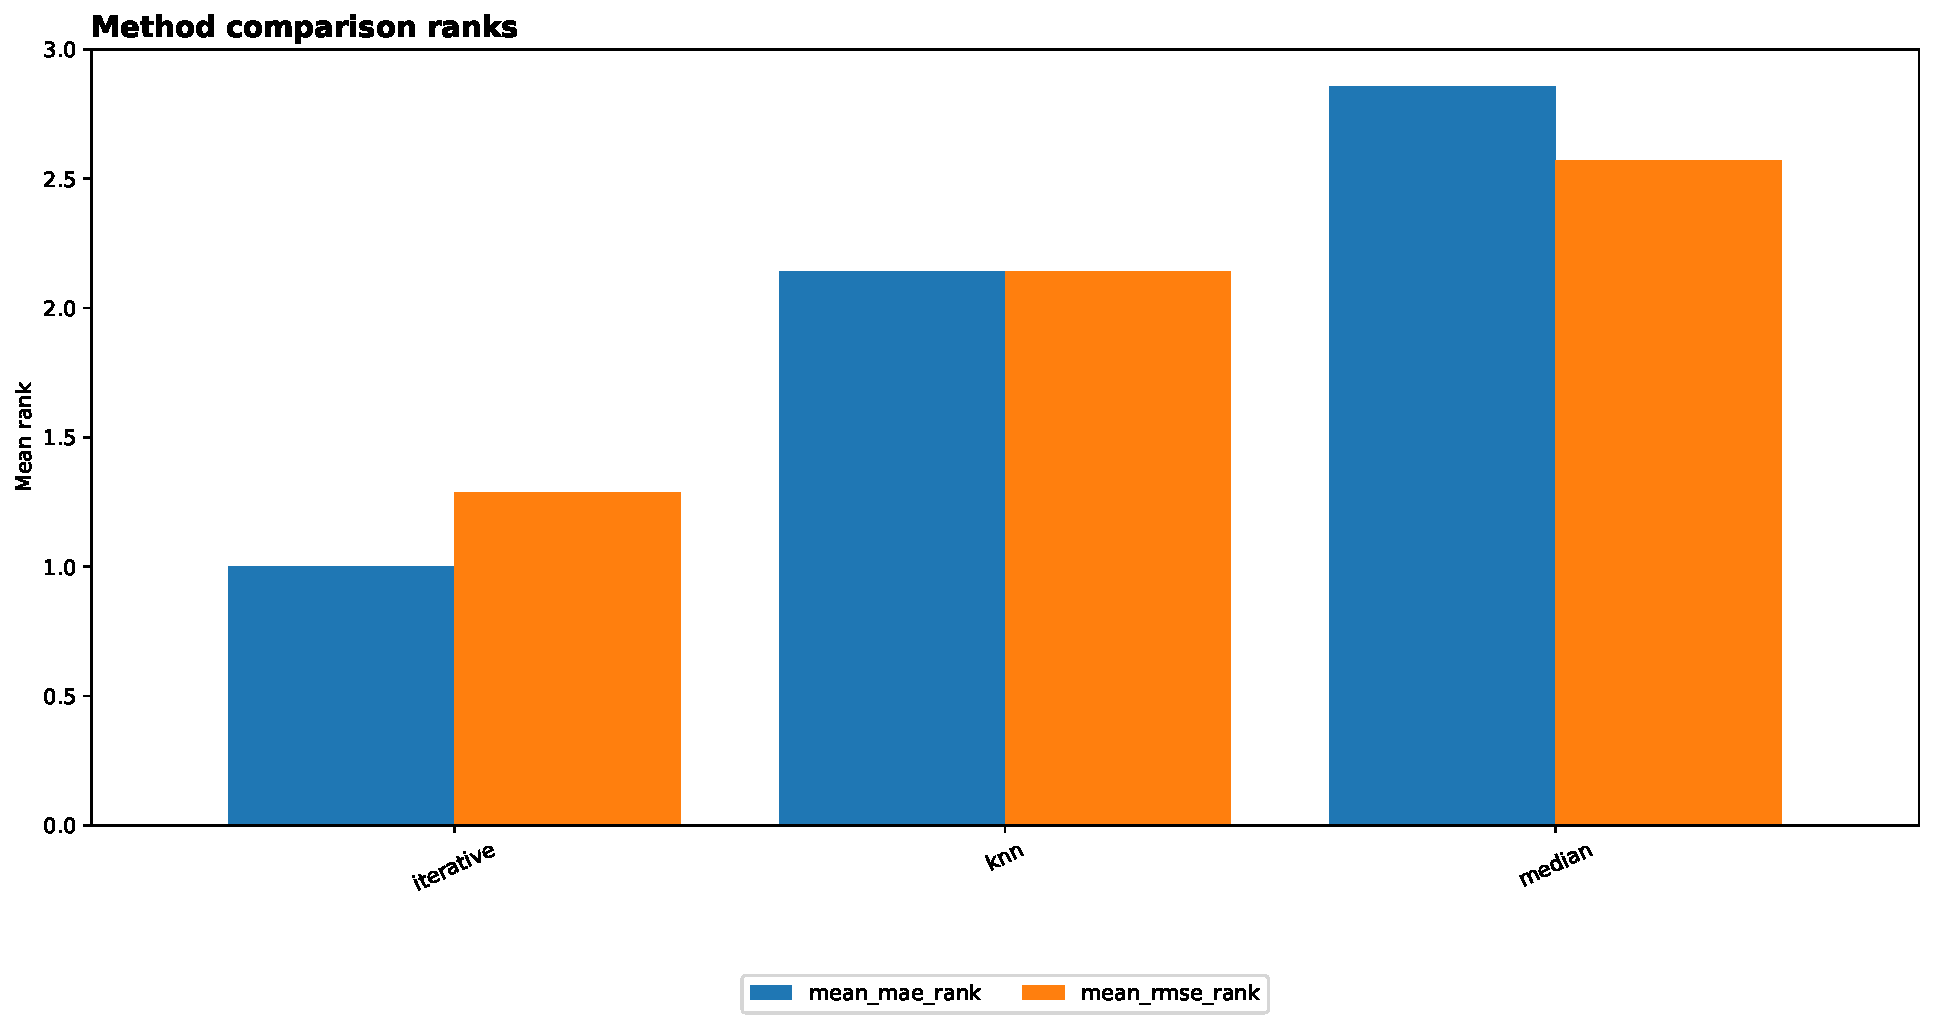
\includegraphics[width=\linewidth]{../../reports/imputation/outputs/figures_pdf/06_method_comparison.pdf}
\caption{Comparacion agregada de metodos por ranks de error.}
\end{figure}

Esta figura justifica la decision de visualizar \method{}. El criterio no es
``\method{} es verdadero'', sino:
\[
  \bar{r}_{\mathrm{MAE}}(\text{iterative})=1.0
  <
  \bar{r}_{\mathrm{MAE}}(\text{knn})
  <
  \bar{r}_{\mathrm{MAE}}(\text{median}).
\]
El metodo iterativo es, en promedio, el que mejor reconstruye valores
ocultados. La interpretacion topologica sigue requiriendo comparar contra KNN
y casos completos.

\subsection{PDFs \code{07}--\code{13}: distribuciones univariadas}

\begin{figure}[H]
\centering
\begin{subfigure}{0.48\linewidth}
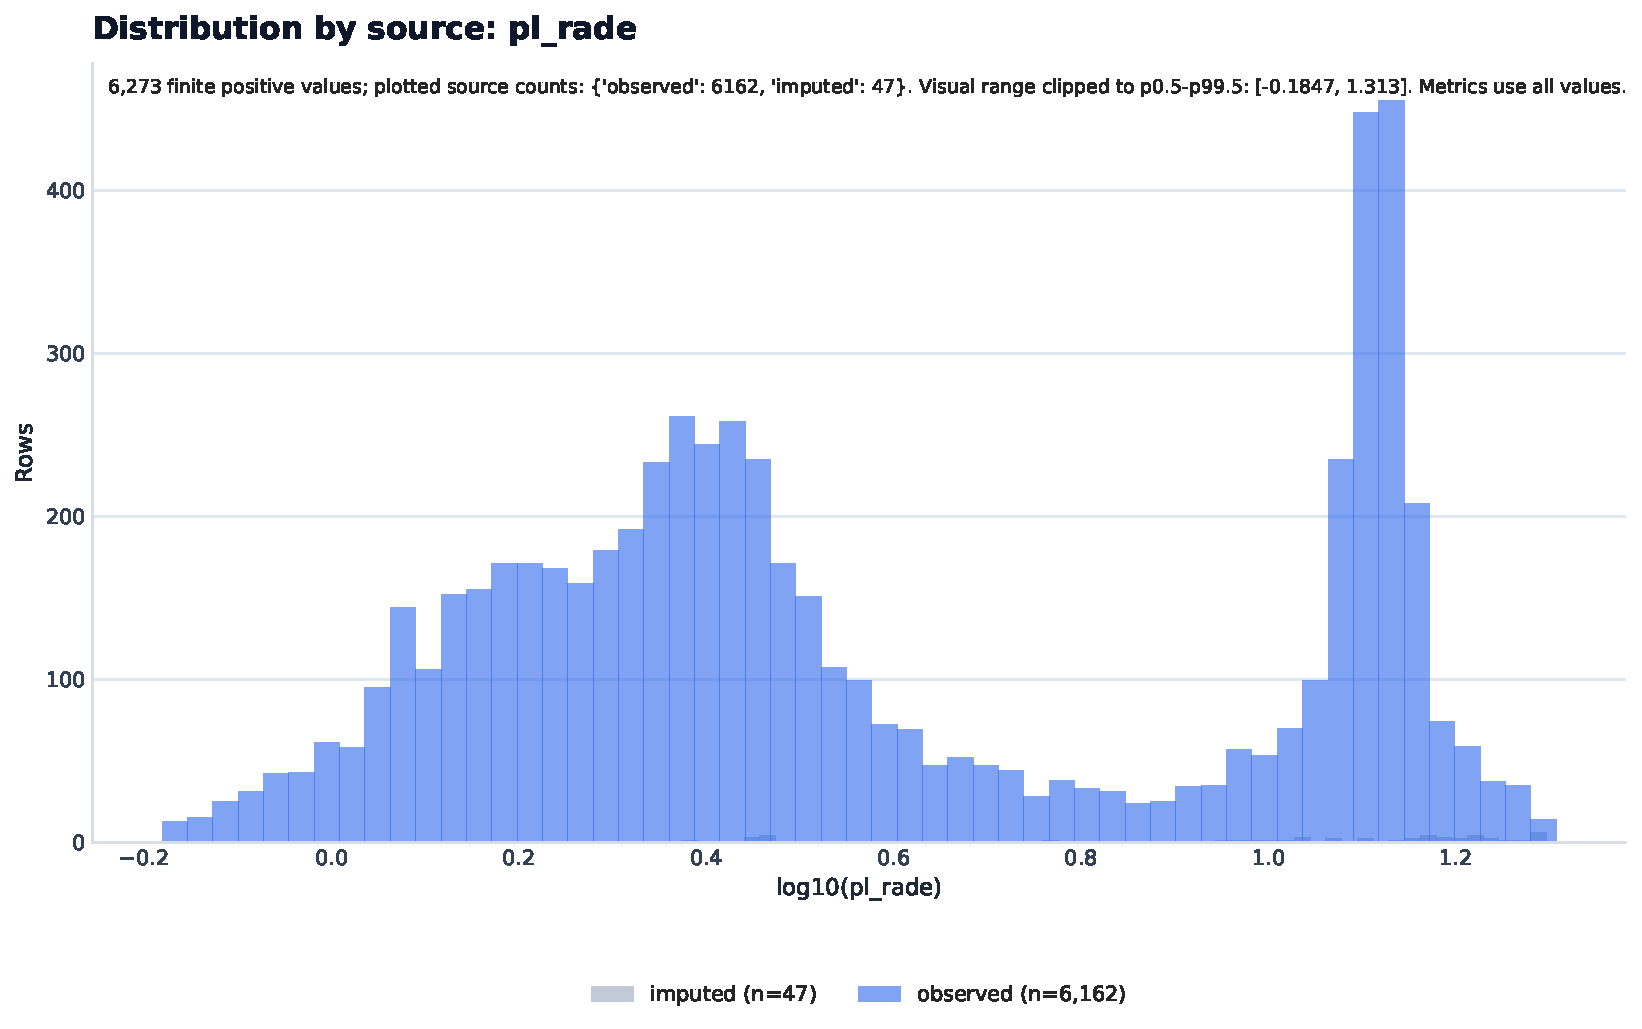
\includegraphics[width=\linewidth]{../../reports/imputation/outputs/figures_pdf/07_distribution_pl_rade.pdf}
\caption{\code{pl\_rade}}
\end{subfigure}
\hfill
\begin{subfigure}{0.48\linewidth}
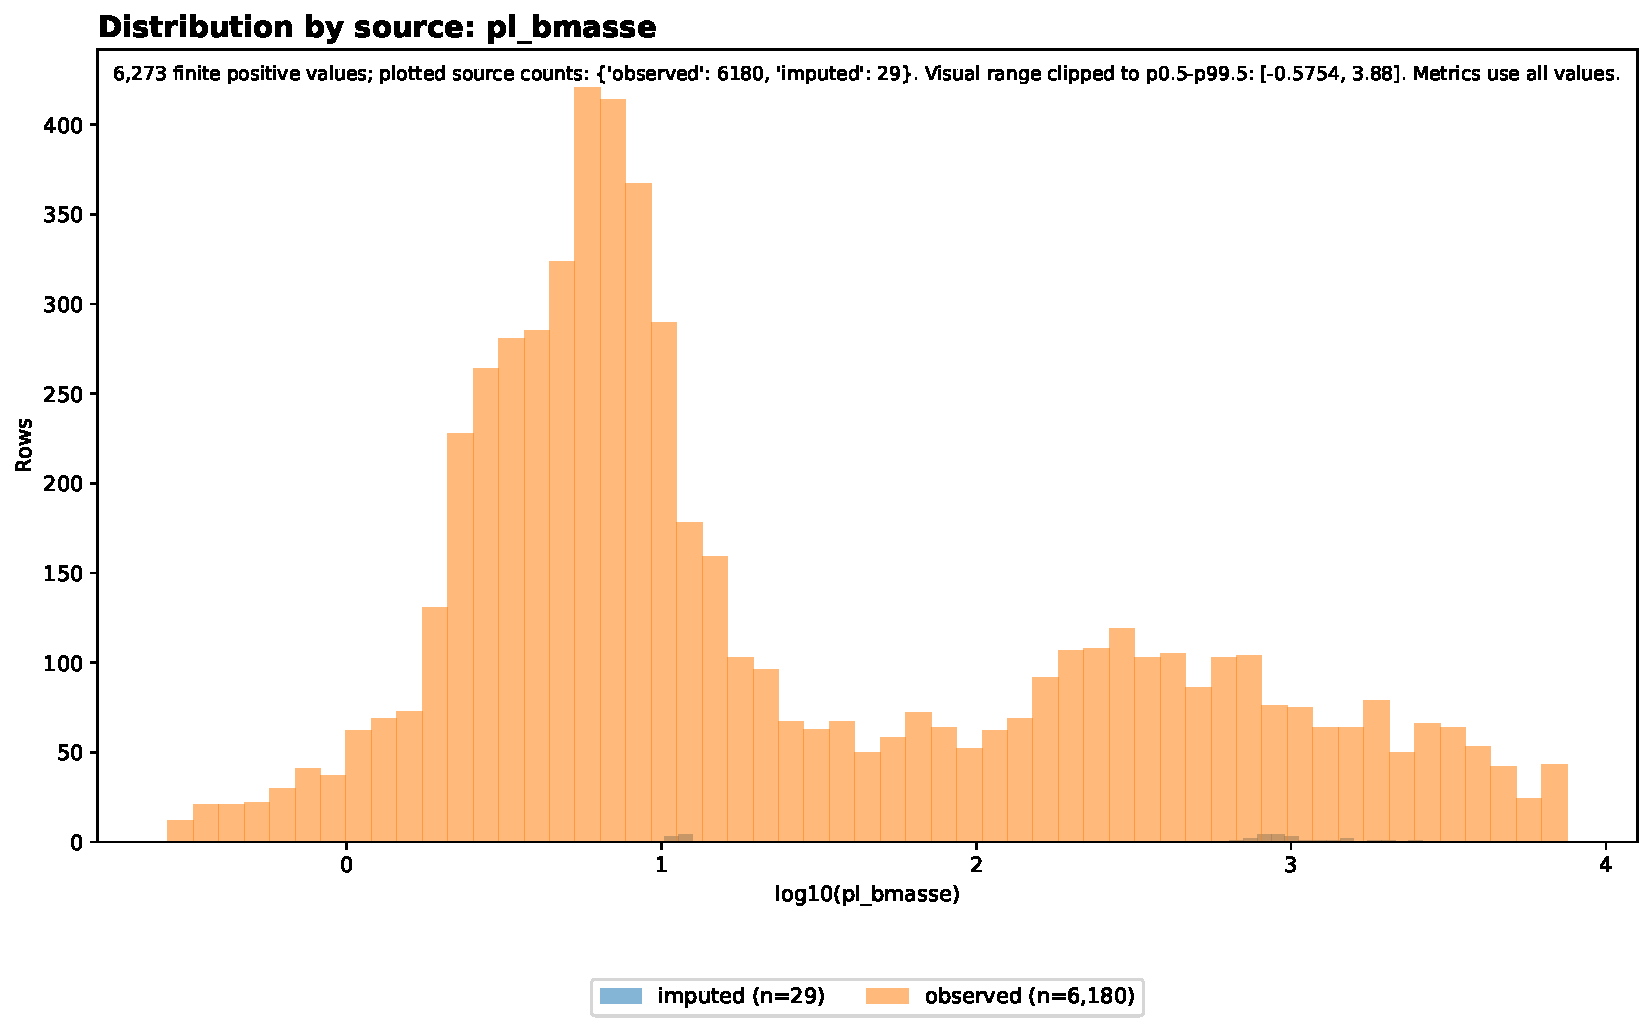
\includegraphics[width=\linewidth]{../../reports/imputation/outputs/figures_pdf/08_distribution_pl_bmasse.pdf}
\caption{\code{pl\_bmasse}}
\end{subfigure}

\begin{subfigure}{0.48\linewidth}
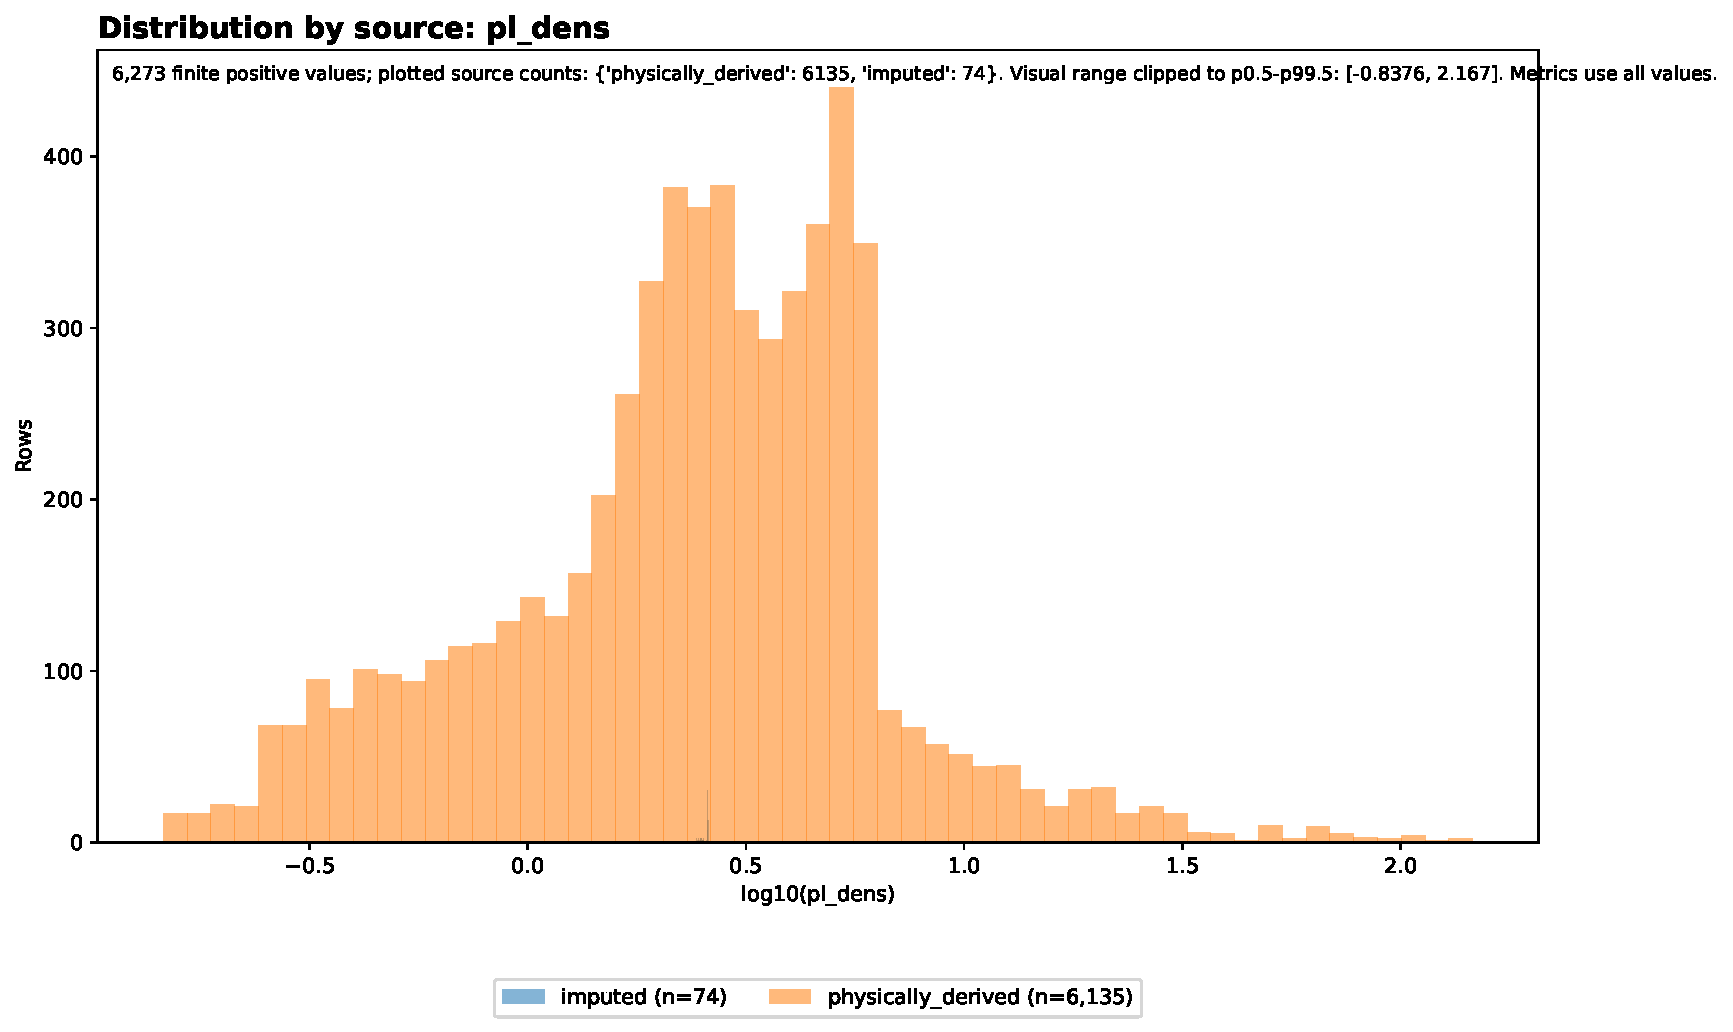
\includegraphics[width=\linewidth]{../../reports/imputation/outputs/figures_pdf/09_distribution_pl_dens.pdf}
\caption{\code{pl\_dens}}
\end{subfigure}
\hfill
\begin{subfigure}{0.48\linewidth}
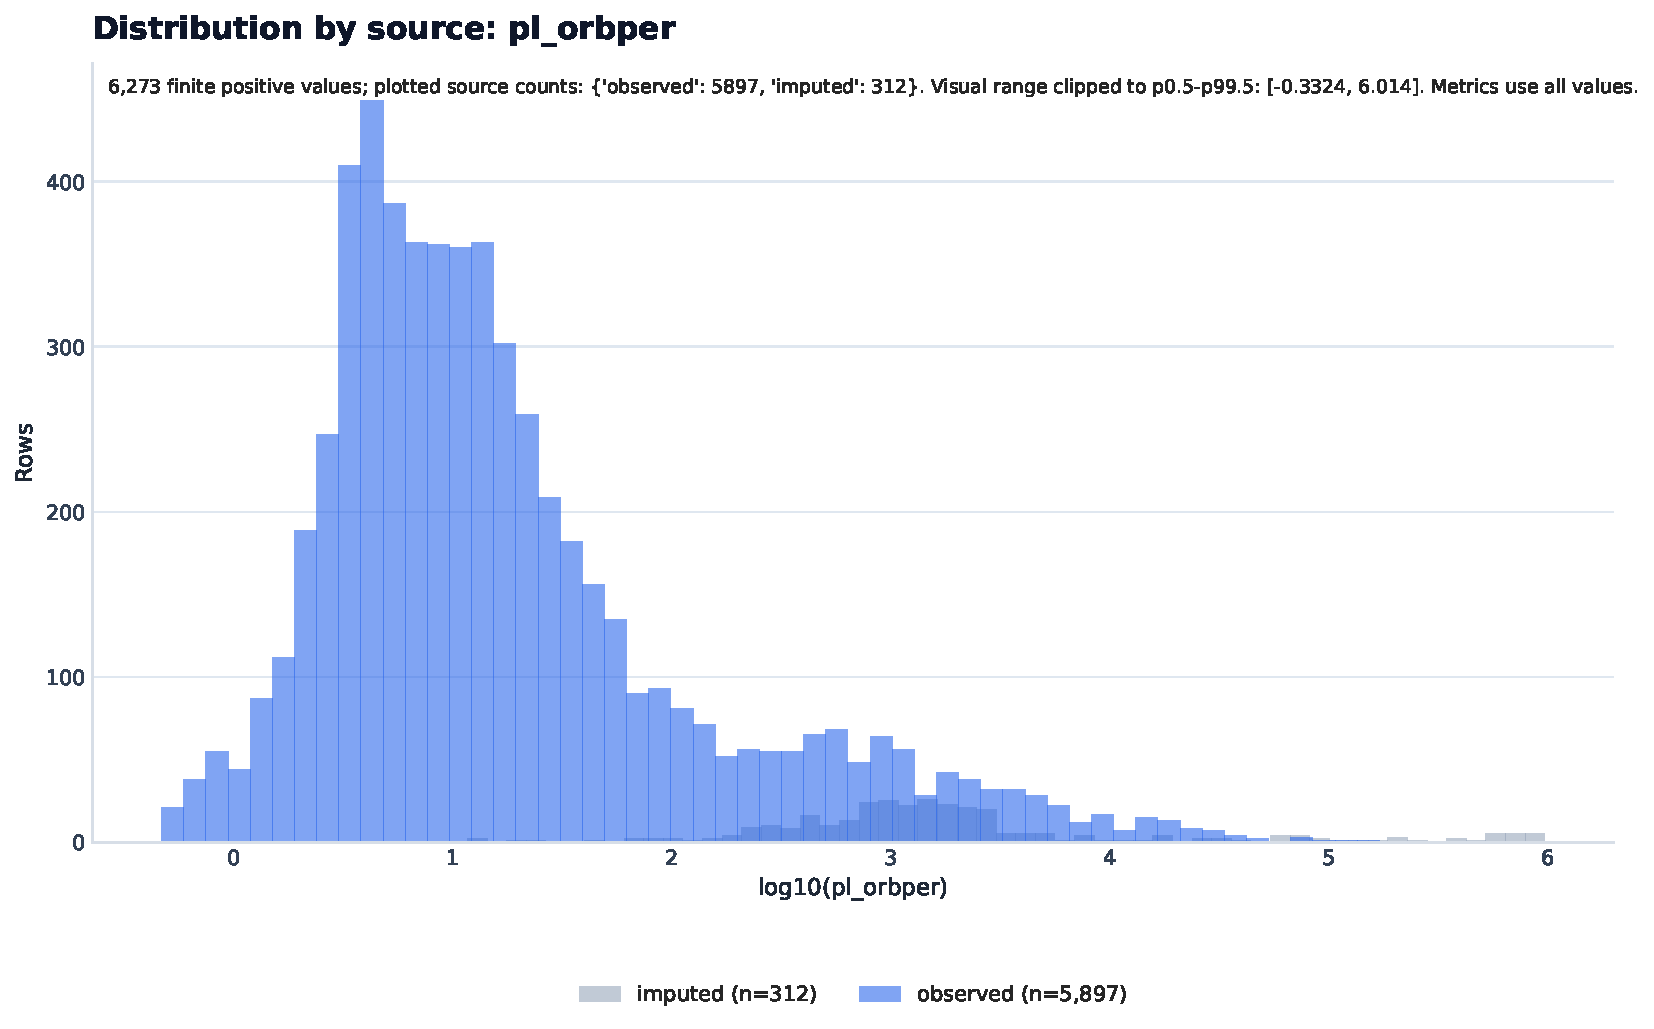
\includegraphics[width=\linewidth]{../../reports/imputation/outputs/figures_pdf/10_distribution_pl_orbper.pdf}
\caption{\code{pl\_orbper}}
\end{subfigure}

\begin{subfigure}{0.48\linewidth}
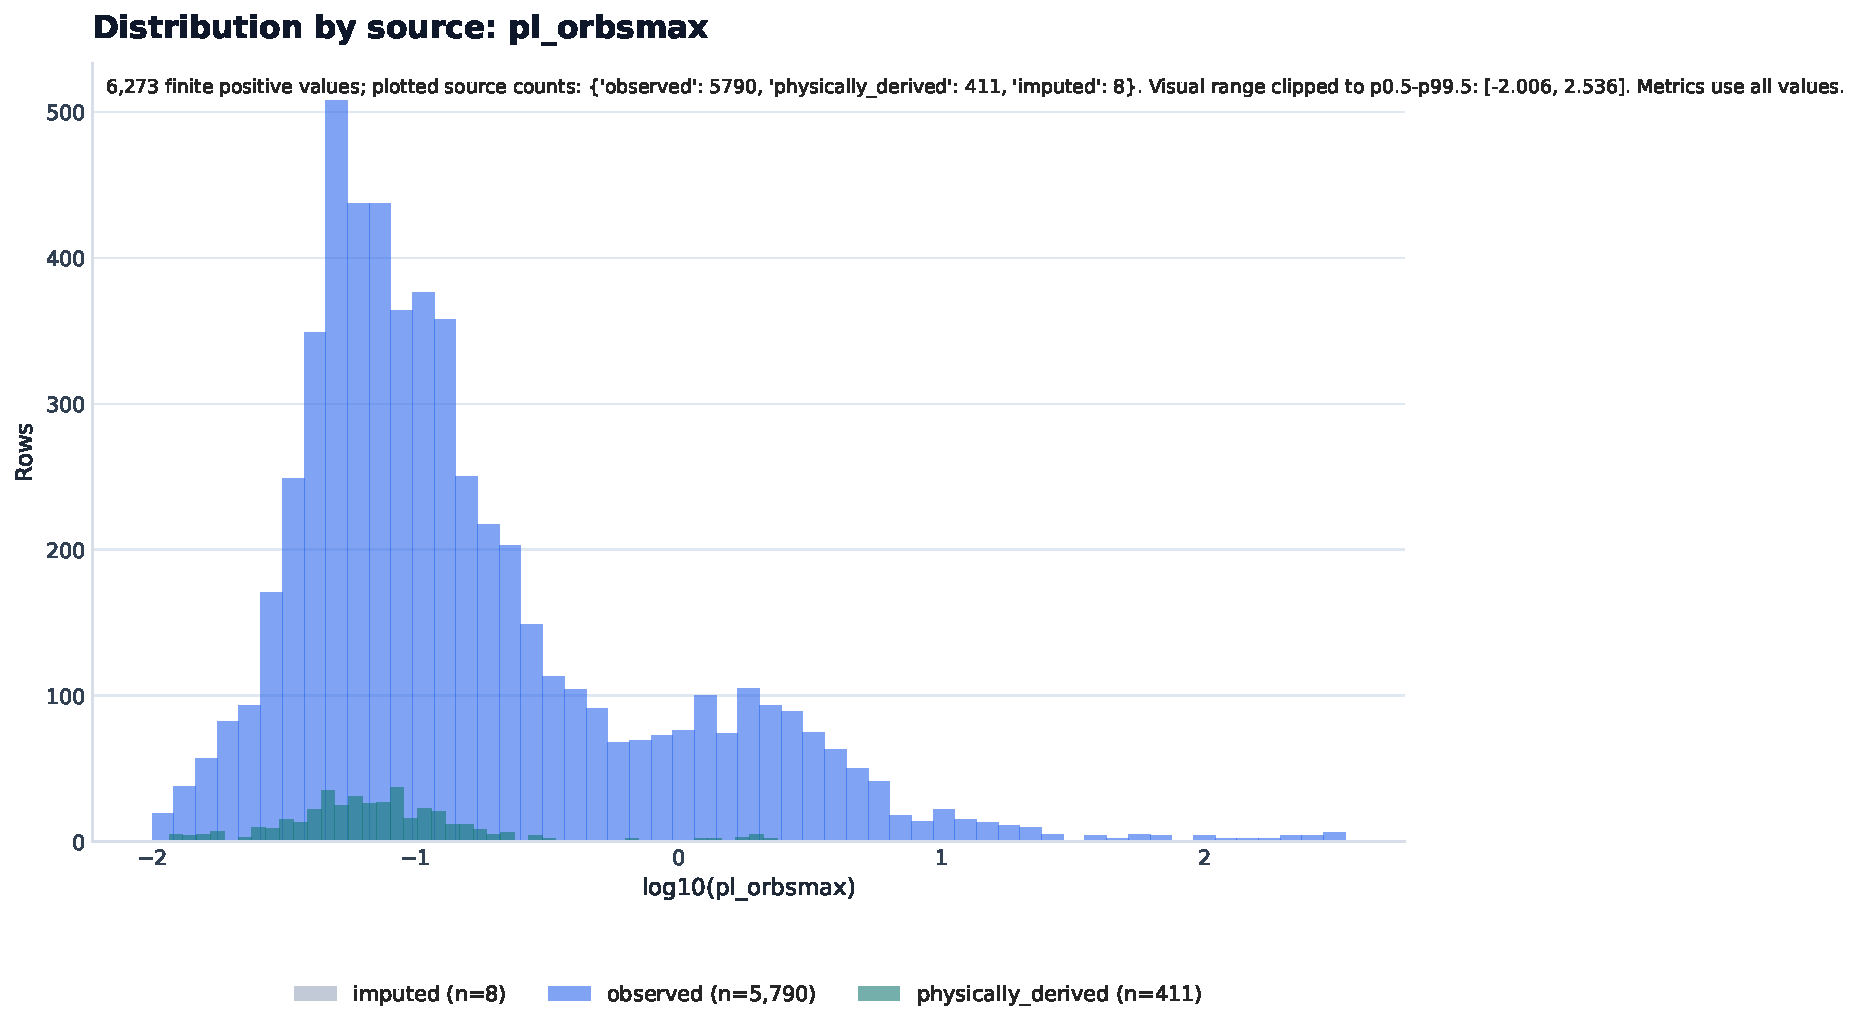
\includegraphics[width=\linewidth]{../../reports/imputation/outputs/figures_pdf/11_distribution_pl_orbsmax.pdf}
\caption{\code{pl\_orbsmax}}
\end{subfigure}
\hfill
\begin{subfigure}{0.48\linewidth}
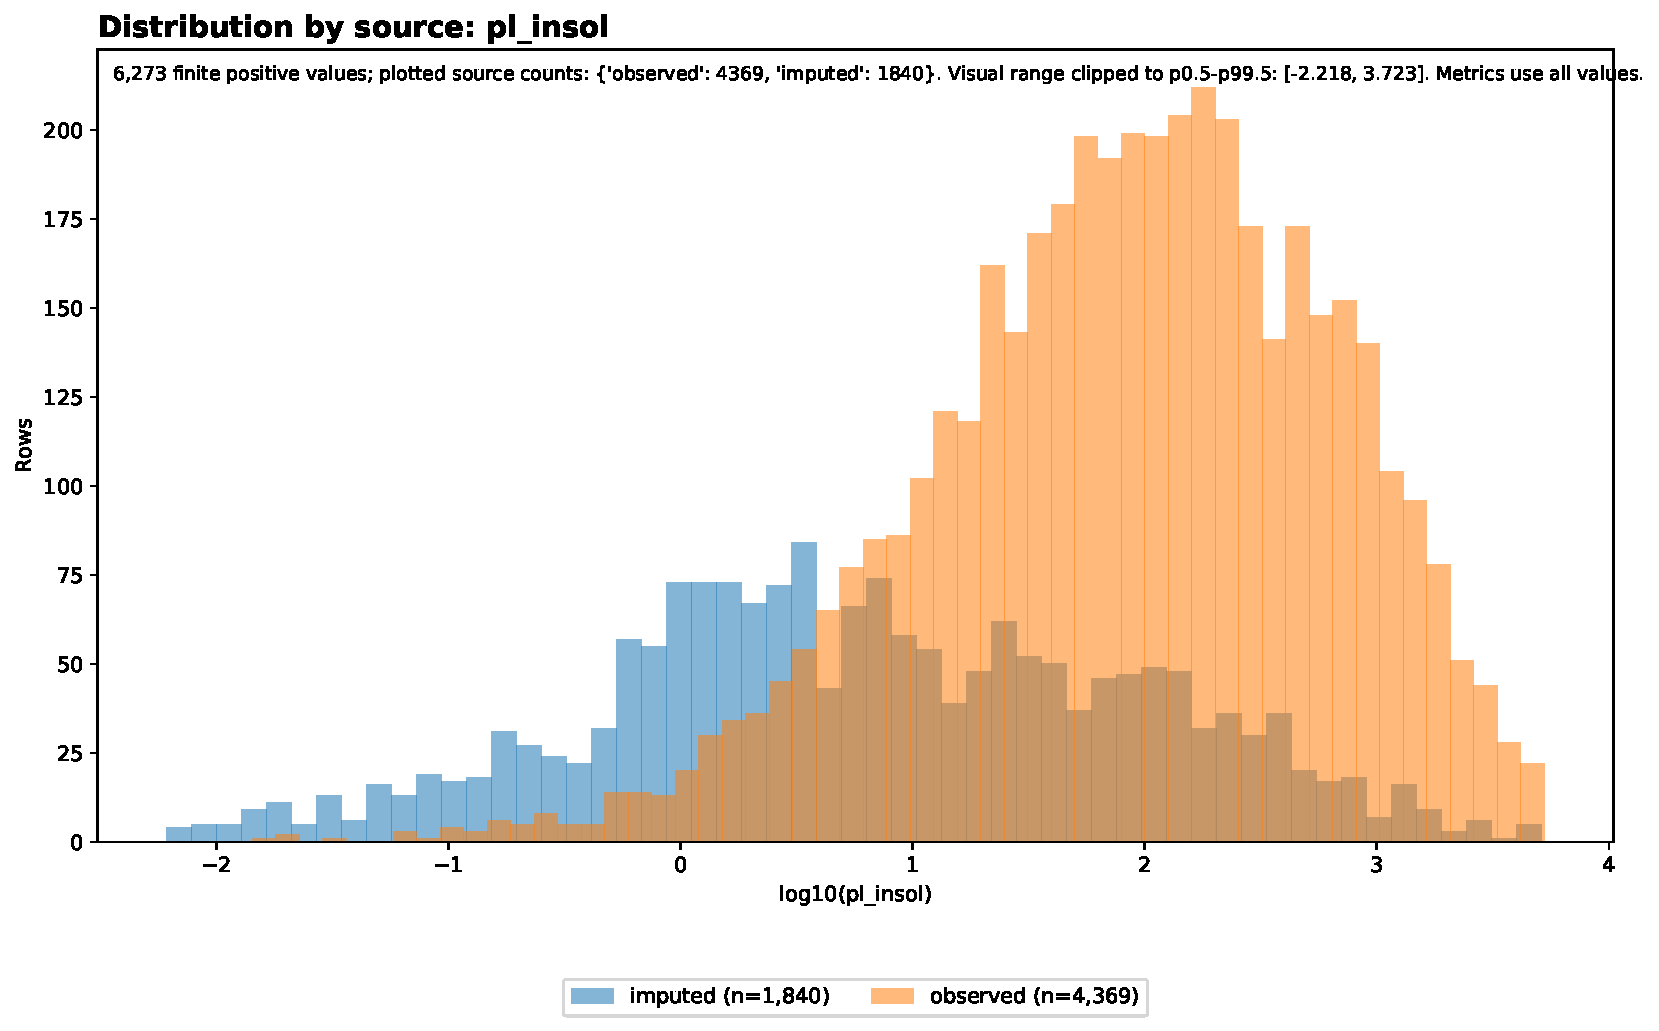
\includegraphics[width=\linewidth]{../../reports/imputation/outputs/figures_pdf/12_distribution_pl_insol.pdf}
\caption{\code{pl\_insol}}
\end{subfigure}

\begin{subfigure}{0.48\linewidth}
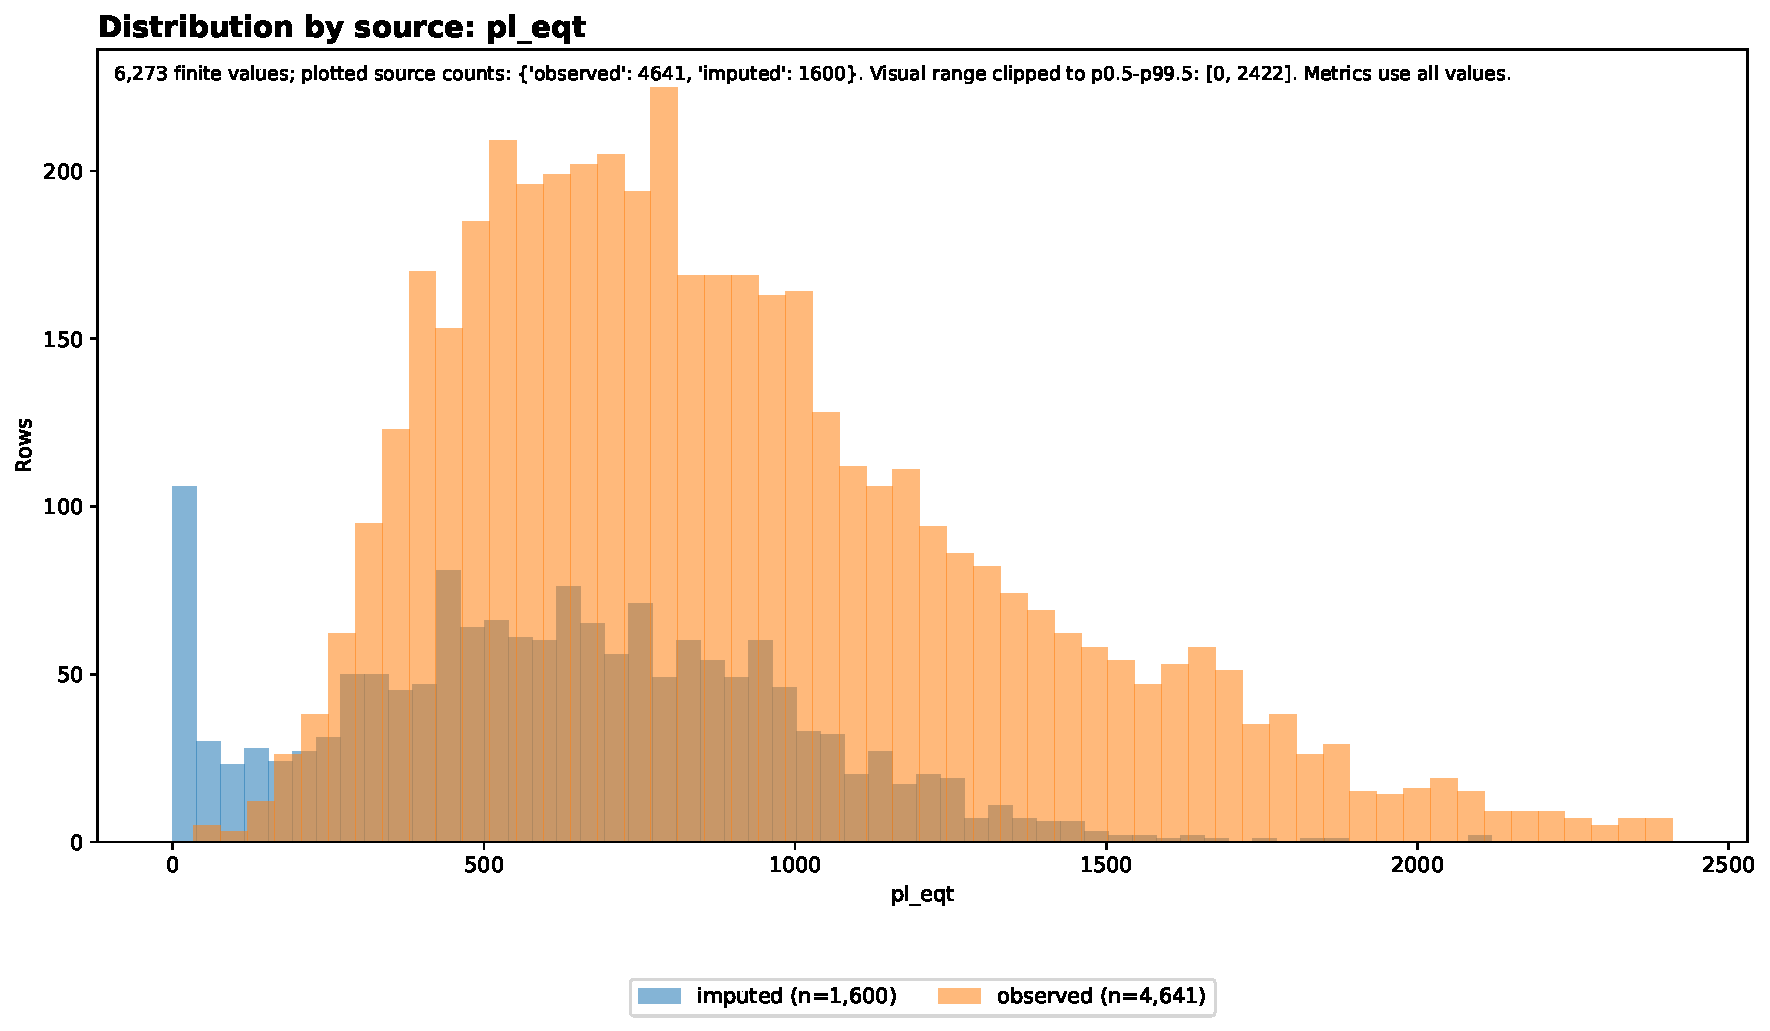
\includegraphics[width=\linewidth]{../../reports/imputation/outputs/figures_pdf/13_distribution_pl_eqt.pdf}
\caption{\code{pl\_eqt}}
\end{subfigure}
\caption{Distribution checks por variable. Las variables positivas de cola larga se leen en escala \(\log_{10}\) cuando corresponde.}
\end{figure}

Estas figuras verifican que las distribuciones no quedaron vacias ni
colapsadas por problemas de escala. Para
\[
  \code{pl\_rade},\code{pl\_bmasse},\code{pl\_dens},
  \code{pl\_orbper},\code{pl\_orbsmax},\code{pl\_insol},
\]
la lectura correcta usa \(\log_{10}(\cdot)\) porque los rangos fisicos son muy
asimetrico. La pregunta diagnostica no es si la distribucion imputada es
identica a la observada, sino si:
\[
  \widehat{p}(x\mid\mathrm{imputed})
\]
cae en regiones plausibles de
\[
  \widehat{p}(x\mid\mathrm{observed\ or\ physically\ derived}).
\]
Si aparecieran masas, radios, densidades, periodos o insolaciones fuera de
ordenes de magnitud razonables, habria que revisar clipping, transformaciones
o el imputador.

\paragraph{\code{pl\_rade}.}
Debe mostrar radios positivos y una distribucion dominada por observados,
porque solo se imputaron 50 de 6273 filas. La imputacion aqui es de bajo peso
relativo.

\paragraph{\code{pl\_bmasse}.}
Debe leerse en log por la cola de masas. Solo 31 filas fueron imputadas, pero
los errores absolutos pueden ser grandes porque masas planetarias tienen rango
amplio.

\paragraph{\code{pl\_dens}.}
La figura no representa observaciones originales de densidad; representa
principalmente densidad derivada:
\[
  6199\ \text{derivadas},\quad 74\ \text{imputadas}.
\]
Su interpretacion es fisico-algebraica, no observacional directa.

\paragraph{\code{pl\_orbper}.}
El periodo orbital requiere escala logaritmica por la presencia de colas muy
largas. Los 339 imputados deben caer en continuidad con periodos observados.

\paragraph{\code{pl\_orbsmax}.}
La mayor parte faltante se resolvio con Kepler, no con imputacion estadistica.
Solo 8 filas quedaron imputadas despues de derivacion.

\paragraph{\code{pl\_insol}.}
Tiene 1876 imputaciones, una proporcion grande. La distribucion debe
inspeccionarse con cuidado porque la insolacion entra a relaciones fisicas con
temperatura de equilibrio y distancia orbital.

\paragraph{\code{pl\_eqt}.}
No usa log en el pipeline. Tiene 1600 imputaciones; por tanto cualquier patron
termico posterior debe distinguir observados de imputados.

\subsection{PDFs \code{14}--\code{17}: scatter checks bivariados}

\begin{figure}[H]
\centering
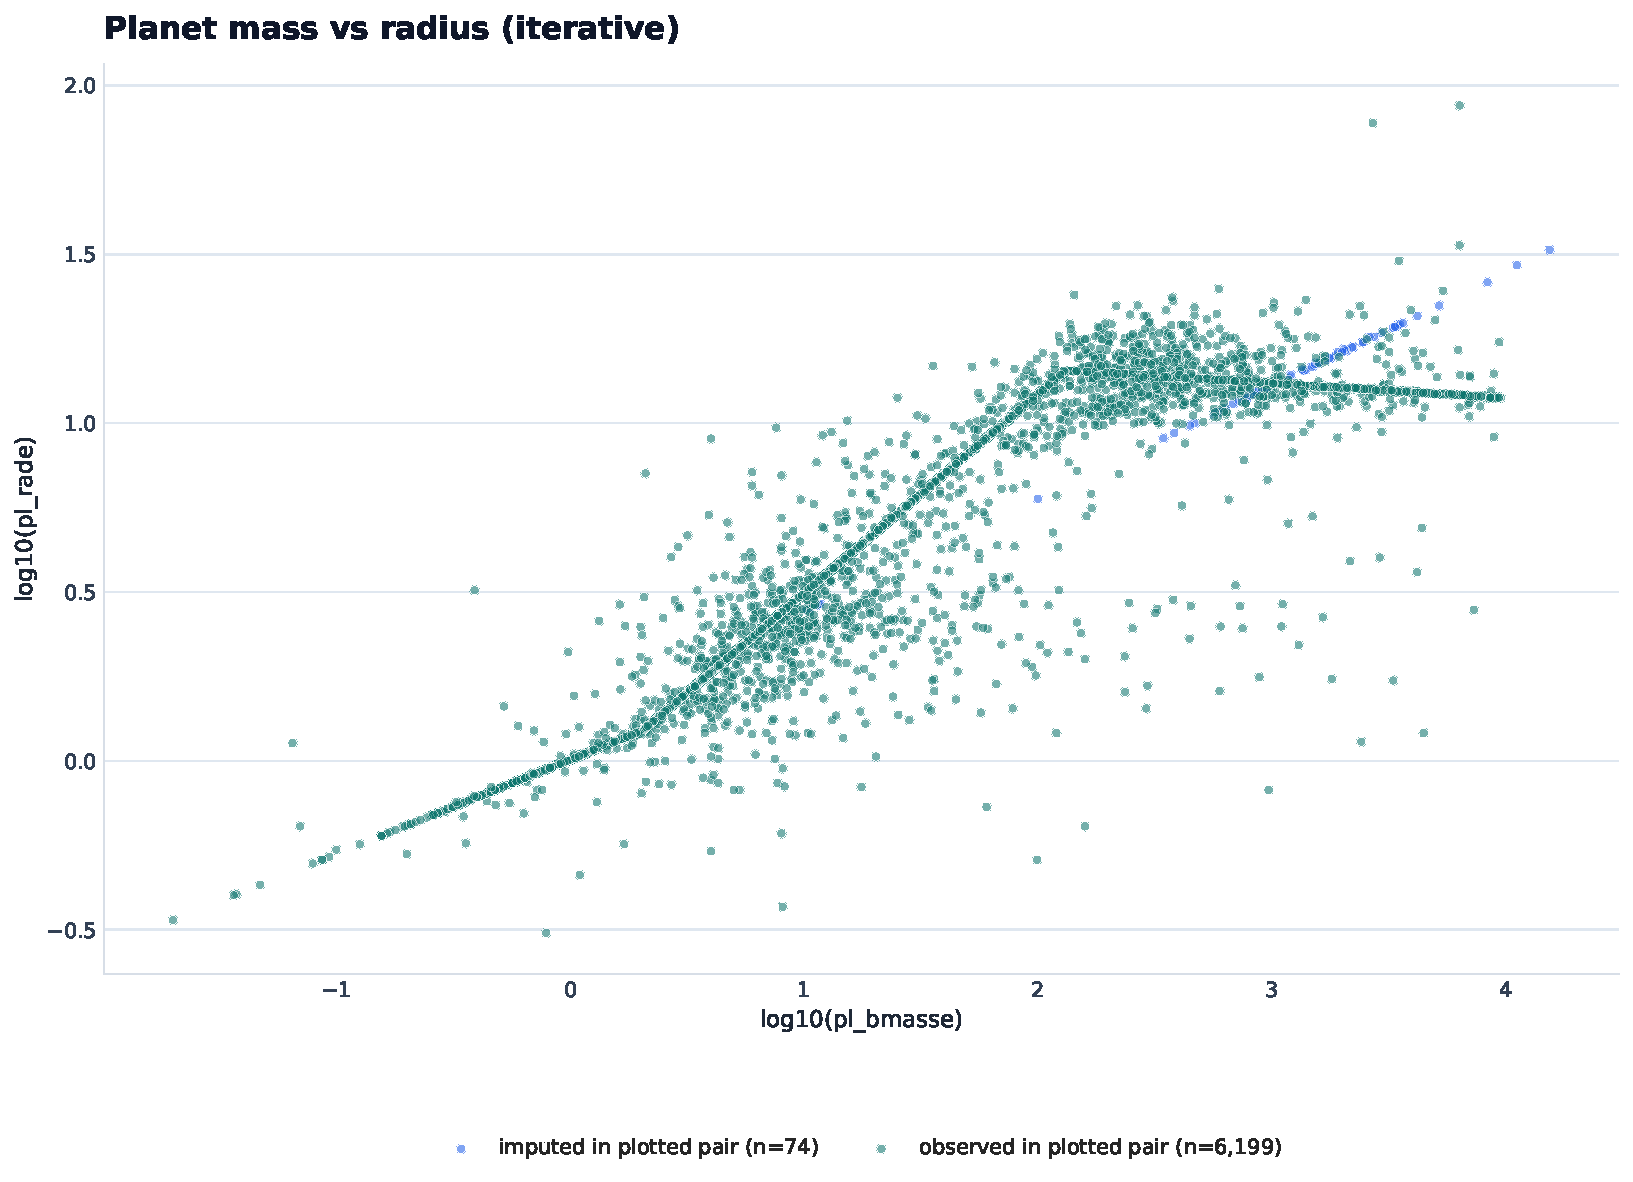
\includegraphics[width=\linewidth]{../../reports/imputation/outputs/figures_pdf/14_scatter_mass_radius.pdf}
\caption{Masa vs radio, coloreado por estatus de imputacion, metodo \method.}
\end{figure}

La relacion masa-radio es el control fisico basico. En escala log-log se
espera una nube amplia, con transiciones entre planetas rocosos, sub-Neptunos,
gigantes gaseosos y objetos masivos. La interpretacion de color es:
\[
  \mathrm{status}(i)
  =
  \begin{cases}
    \text{observed pair}, & x_i,y_i\ \text{observados},\\
    \text{physically derived in plotted pair}, & \exists\ \text{coordenada derivada},\\
    \text{imputed in plotted pair}, & \exists\ \text{coordenada imputada}.
  \end{cases}
\]
Los puntos imputados no deben formar una nube artificial separada sin soporte
observacional.

\begin{figure}[H]
\centering
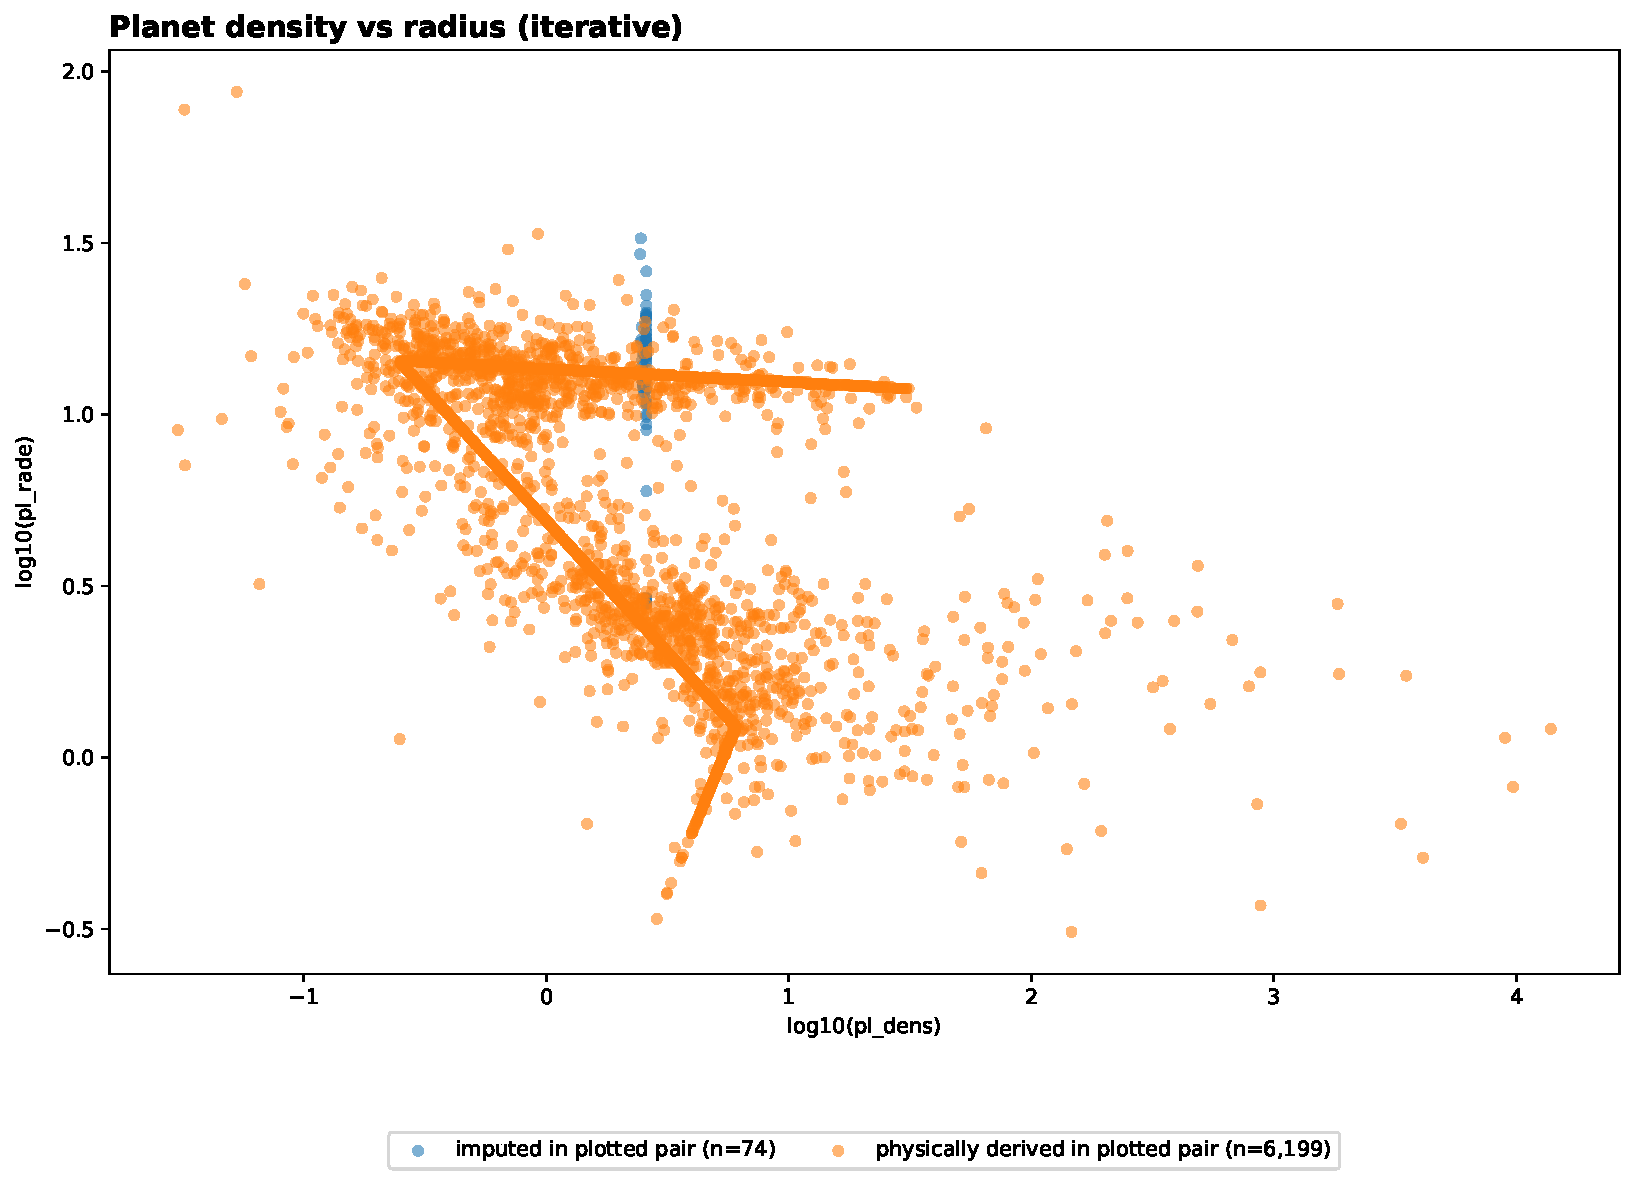
\includegraphics[width=\linewidth]{../../reports/imputation/outputs/figures_pdf/15_scatter_density_radius.pdf}
\caption{Densidad vs radio, coloreado por estatus de imputacion, metodo \method.}
\end{figure}

Este scatter es particularmente delicado porque
\[
  \rho_p \propto \frac{M_p}{R_p^3}.
\]
Al poner \(\rho_p\) contra \(R_p\), parte de la estructura visual esta inducida
por la formula misma. Si \code{pl\_dens} fue derivada desde masa y radio, no es
una coordenada independiente. Por eso el plot sirve para detectar coherencia
fisica y outliers, no para afirmar una correlacion observacional independiente
entre densidad y radio.

\begin{figure}[H]
\centering
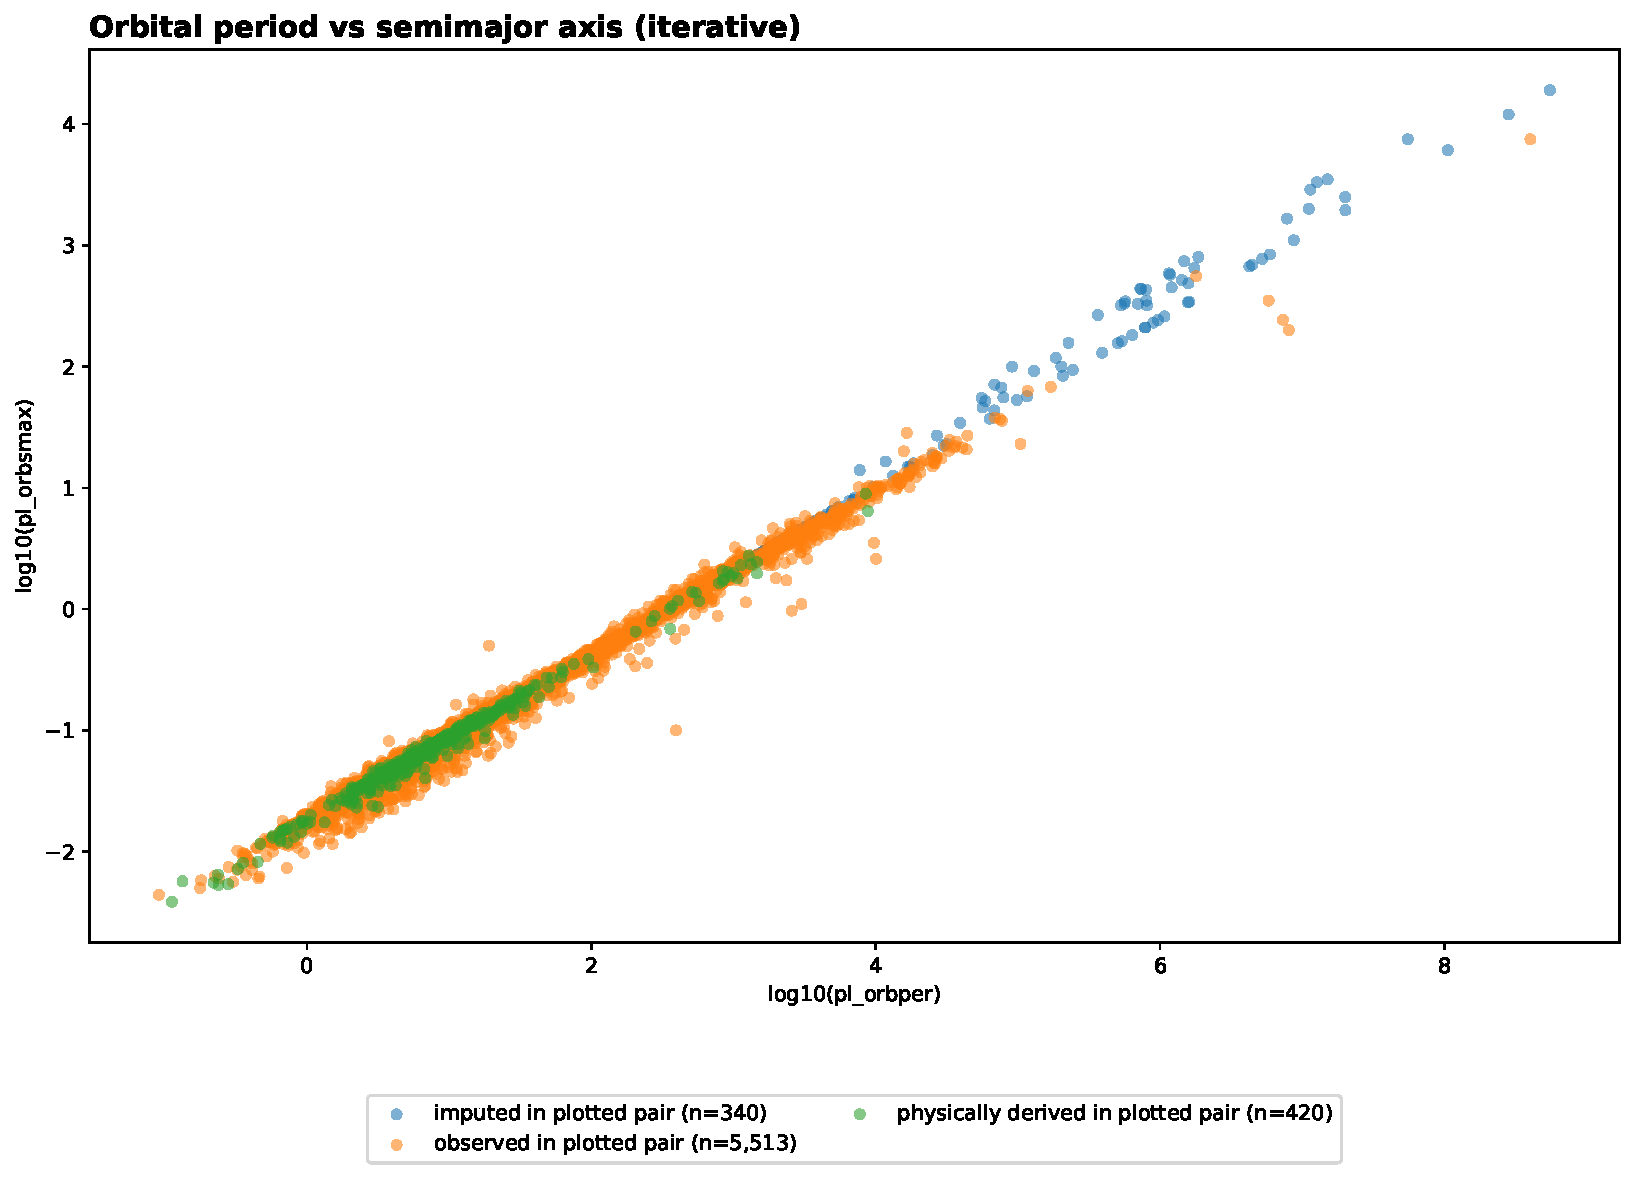
\includegraphics[width=\linewidth]{../../reports/imputation/outputs/figures_pdf/16_scatter_orbper_orbsmax.pdf}
\caption{Periodo orbital vs semieje mayor, coloreado por estatus de imputacion, metodo \method.}
\end{figure}

Este scatter debe reflejar la relacion kepleriana:
\[
  a \propto M_\star^{1/3} P^{2/3}.
\]
En logaritmos:
\[
  \log a
  =
  \frac{1}{3}\log M_\star
  +
  \frac{2}{3}\log P
  -
  \frac{2}{3}\log 365.25.
\]
Por tanto, una estructura aproximadamente monotona no es sorpresa; esta
parcialmente inducida cuando \code{pl\_orbsmax} fue derivado. El valor del plot
es verificar que los pocos imputados estadisticamente no rompan esta relacion.

\begin{figure}[H]
\centering
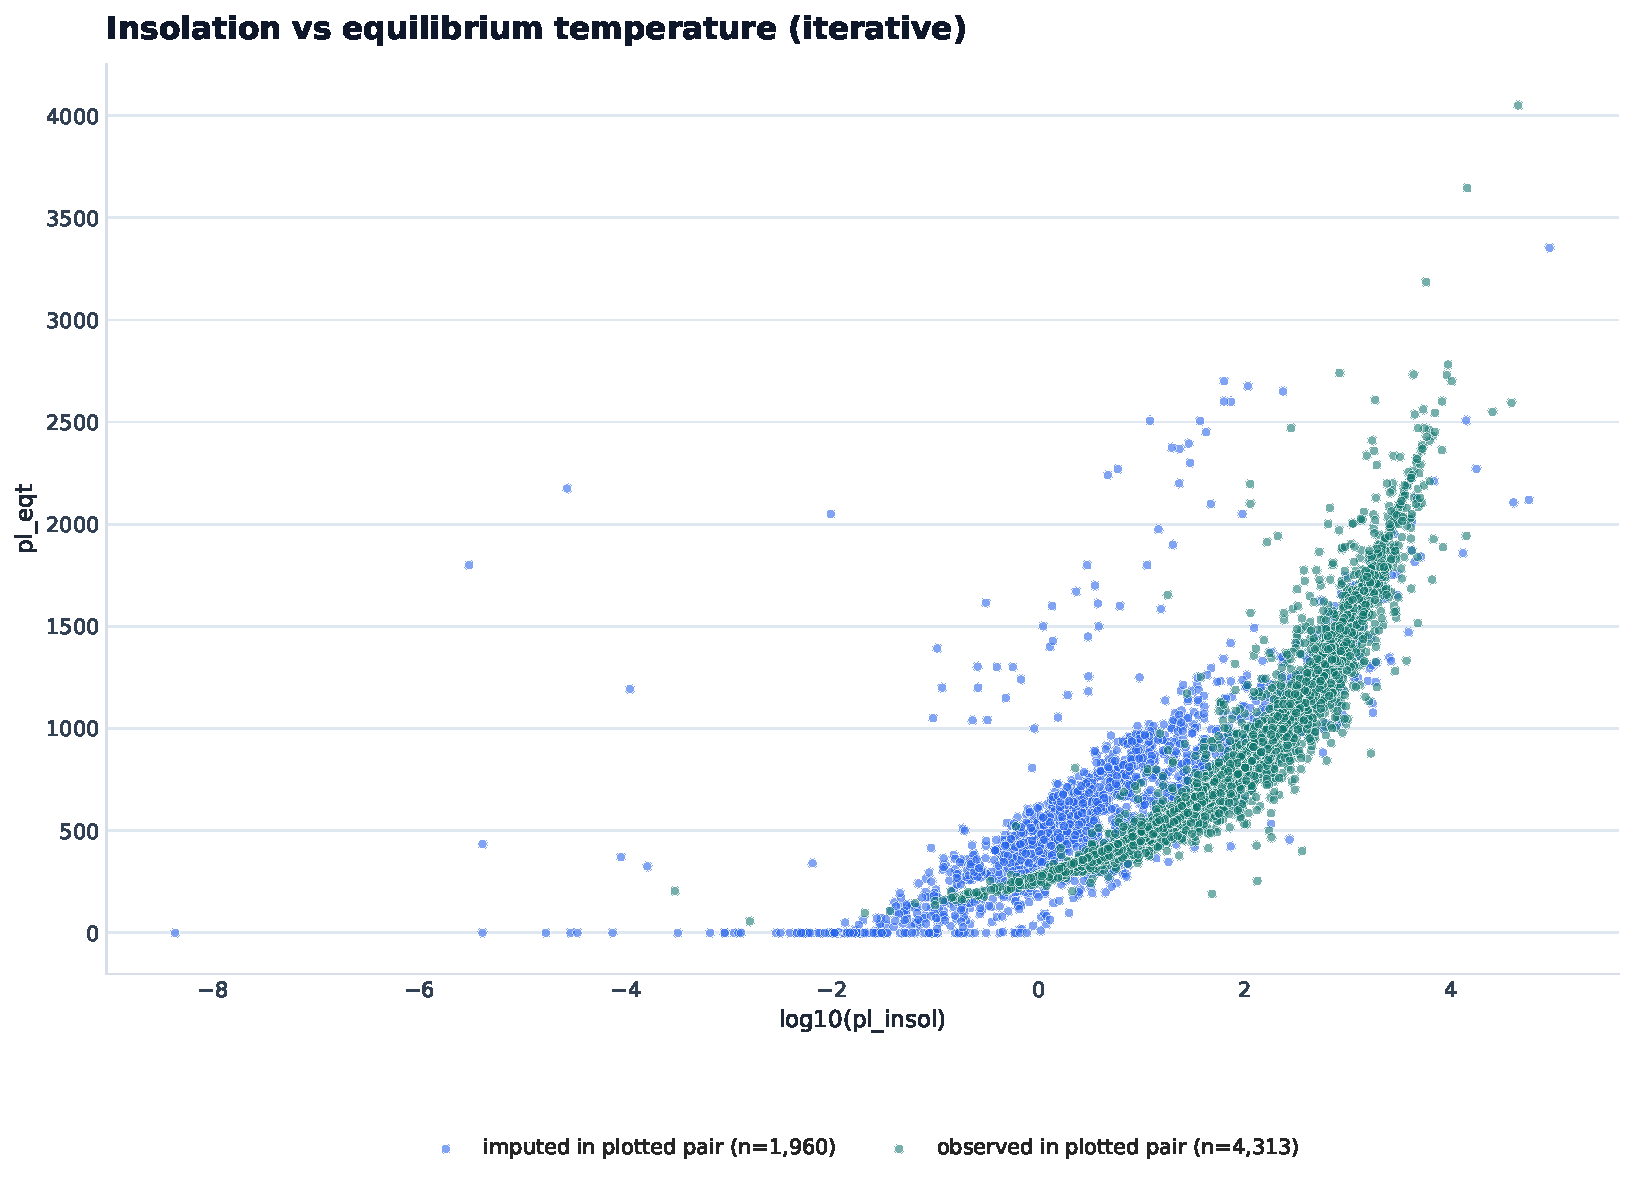
\includegraphics[width=\linewidth]{../../reports/imputation/outputs/figures_pdf/17_scatter_insol_eqt.pdf}
\caption{Insolacion vs temperatura de equilibrio, coloreado por estatus de imputacion, metodo \method.}
\end{figure}

La temperatura de equilibrio e insolacion estan fisicamente relacionadas. De
forma idealizada:
\[
  T_{\mathrm{eq}}
  \propto
  S^{1/4},
\]
si se mantienen constantes albedo y redistribucion termica. En logaritmos:
\[
  \log T_{\mathrm{eq}}
  =
  C + \frac{1}{4}\log S.
\]
Como \code{pl\_insol} tiene 1876 imputaciones y \code{pl\_eqt} tiene 1600,
este scatter es un diagnostico de coherencia termica del imputador
\method{}. Si los puntos imputados se alinean razonablemente con la nube
principal, el metodo preserva una relacion fisica esperada; si se separan,
habria sesgo en variables termicas.

\section{Lectura de tablas exportadas}

Las tablas principales exportadas en CSV y JSON son:
\begin{itemize}
  \item \code{imputation\_method\_comparison}.
  \item \code{imputation\_validation\_metrics}.
  \item \code{imputation\_value\_source\_composition}.
  \item \code{imputation\_missingness\_summary}.
  \item \code{mapper\_coverage\_summary}.
\end{itemize}

\subsection{\code{imputation\_method\_comparison}}

Esta tabla no debe interpretarse como prueba ontologica de que un metodo es
``correcto''. Es una comparacion empirica bajo mascara aleatoria:
\[
  m^\star
  =
  \arg\min_m
  \left[
    \bar{r}_{\mathrm{MAE}}(m)
  \right].
\]
El resultado favorece \method{} por error promedio, pero no elimina la
necesidad de sensibilidad topologica.

\subsection{\code{imputation\_validation\_metrics}}

La columna mas importante conceptualmente es
\code{validation\_basis}. En particular:
\[
  \code{pl\_dens}:\quad
  \code{validation\_basis}=\text{physically\_derived}.
\]
Esto significa que al ocultar y reconstruir \code{pl\_dens}, la verdad
comparativa era la densidad calculada por formula, no una medicion original.

\subsection{\code{imputation\_value\_source\_composition}}

Esta tabla es la auditoria de procedencia. Debe acompanar cualquier analisis
posterior porque permite filtrar o ponderar:
\[
  \widehat{X}_{\mathrm{obs}},\quad
  \widehat{X}_{\mathrm{phys}},\quad
  \widehat{X}_{\mathrm{imp}}.
\]
Para un analisis conservador se pueden comparar resultados usando:
\[
  \{\text{observed}\}
  \quad\text{vs.}\quad
  \{\text{observed},\text{physically\_derived}\}
  \quad\text{vs.}\quad
  \{\text{observed},\text{physically\_derived},\text{imputed}\}.
\]

\subsection{\code{imputation\_missingness\_summary}}

Esta tabla documenta en que etapa se resolvio cada hueco. Es crucial porque
\code{pl\_dens} parece inicialmente inutilizable al estar \(100\%\) faltante,
pero se vuelve casi completa despues de derivacion fisica.

\subsection{\code{mapper\_coverage\_summary}}

Esta tabla conecta imputacion con TDA. El salto de cobertura del espacio
conjunto:
\[
  4282 \to 6273
\]
indica cuantas filas adicionales entran al grafo Mapper gracias al pipeline.
Esa ganancia de cobertura es util, pero cambia la distribucion geometrica del
espacio analizado.

\section{Implicaciones para Mapper/TDA}

Mapper no opera sobre los datos crudos directamente, sino sobre una nube
\[
  \mathcal{X}
  =
  \{\widehat{\mathbf{x}}_1,\dots,\widehat{\mathbf{x}}_n\}
  \subset \R^p
\]
despues de transformacion, escalado e imputacion. Una lente
\[
  f:\mathcal{X}\to\R^d
\]
define una cubierta \(\mathcal{U}\) del espacio de lentes; luego se agrupan
puntos en preimagenes \(f^{-1}(U_\alpha)\), y se construye un grafo por
interseccion de clusters. Por tanto, pequenas perturbaciones en
\(\widehat{\mathbf{x}}_i\) pueden alterar:
\[
  f(\widehat{\mathbf{x}}_i),\quad
  \mathrm{cluster}(\widehat{\mathbf{x}}_i),\quad
  E(G_{\mathrm{Mapper}}).
\]

El pipeline mejora cobertura:
\[
  \mathrm{coverage}_{\mathrm{joint}}=100\%.
\]
Pero la estabilidad topologica debe evaluarse con comparaciones:
\[
  G_{\mathrm{complete}},
  \quad
  G_{\mathrm{median}},
  \quad
  G_{\mathrm{knn}},
  \quad
  G_{\mathrm{iterative}},
  \quad
  G_{\mathrm{bootstrap}},
  \quad
  G_{\mathrm{params}}.
\]
Una conclusion topologica fuerte deberia persistir bajo varias de estas
condiciones.

\section{Criterios de aceptacion cumplidos}

\begin{enumerate}
  \item El HTML final contiene \code{METODO VISUALIZADO = iterative}.
  \item Los plots dependientes del metodo usan \method{}.
  \item Los histogramas/distribuciones no estan vacios por problemas de escala.
  \item Los scatter finales 14--17 usan \method{}.
  \item Hay 17 PDFs individuales en \figdir{} y todos tienen tamano mayor que
  cero.
  \item Las tablas principales existen como CSV y JSON en \tablesdir{}.
  \item El reporte distingue observados, derivados fisicamente e imputados.
  \item \code{pl\_dens} se describe como derivada desde masa y radio cuando
  aplica.
  \item No quedan \(\missing\), \(+\infty\) ni \(-\infty\) en las siete
  features principales para el metodo \method{}.
  \item La estructura del repositorio se mantuvo; no se reescribio el pipeline.
\end{enumerate}

\section{Advertencias no bloqueantes}

La suite de pruebas paso:
\[
  18\ \text{passed},\qquad 1\ \text{warning}.
\]
El warning observado corresponde a carga simultanea de bibliotecas OpenMP
\code{libiomp} y \code{libomp} reportada por \code{threadpoolctl}. Esto es una
advertencia del stack numerico local, no un fallo del pipeline de imputacion.

\section{Conclusiones}

El pipeline final produce una matriz completa para las siete variables Mapper
principales, con trazabilidad explicita de procedencia. La decision de
visualizar \method{} esta respaldada por validacion enmascarada y rank promedio
de error. Sin embargo, el documento conserva la distincion epistemica central:
\[
  \text{observado} \ne \text{derivado fisicamente} \ne \text{imputado}.
\]
En particular,
\[
  \code{pl\_dens}
  =
  5.514\,
  \frac{\code{pl\_bmasse}}{\code{pl\_rade}^{3}}
\]
para 6199 filas, y solo 74 densidades finales provienen de imputacion
estadistica bajo \method{}. Por tanto, cualquier interpretacion fisica o
topologica posterior debe reportar el metodo, las fuentes de valor y la
comparacion contra alternativas.

\appendix
\section{Rutas de artefactos}

\begin{itemize}
  \item HTML final: \code{reports/imputation/imputation\_report.html}.
  \item Figuras PDF: \code{reports/imputation/outputs/figures\_pdf/}.
  \item Tablas CSV/JSON: \code{reports/imputation/outputs/tables/}.
  \item CSV imputado visualizado: \code{reports/imputation/PSCompPars\_imputed\_iterative.csv}.
  \item Features Mapper visualizadas: \code{reports/imputation/mapper\_features\_imputed\_iterative.csv}.
\end{itemize}

\section{Inventario de PDFs}

\begin{center}
\begin{longtable}{lr}
\toprule
PDF & Bytes\\
\midrule
\endhead
\code{01\_missingness\_before\_after.pdf} & 20745\\
\code{02\_value\_source\_composition.pdf} & 19610\\
\code{03\_mapper\_coverage.pdf} & 20873\\
\code{04\_masked\_validation\_mae\_by\_feature.pdf} & 19213\\
\code{05\_masked\_validation\_spearman\_heatmap.pdf} & 21825\\
\code{06\_method\_comparison.pdf} & 16144\\
\code{07\_distribution\_pl\_rade.pdf} & 27262\\
\code{08\_distribution\_pl\_bmasse.pdf} & 27034\\
\code{09\_distribution\_pl\_dens.pdf} & 26821\\
\code{10\_distribution\_pl\_orbper.pdf} & 26234\\
\code{11\_distribution\_pl\_orbsmax.pdf} & 29210\\
\code{12\_distribution\_pl\_insol.pdf} & 26821\\
\code{13\_distribution\_pl\_eqt.pdf} & 26521\\
\code{14\_scatter\_mass\_radius.pdf} & 116627\\
\code{15\_scatter\_density\_radius.pdf} & 116363\\
\code{16\_scatter\_orbper\_orbsmax.pdf} & 119954\\
\code{17\_scatter\_insol\_eqt.pdf} & 111064\\
\bottomrule
\end{longtable}
\end{center}

\end{document}
